\documentclass[conference]{IEEEtran}
\IEEEoverridecommandlockouts

% Basic IEEE packages
\usepackage{cite}
\usepackage{amsmath,amssymb,amsfonts}
\usepackage{graphicx}
\usepackage{textcomp}
\usepackage{xcolor}
\usepackage{booktabs}
\usepackage{array}
\usepackage{url}
\usepackage{subcaption}
\usepackage{multirow}
\usepackage{dblfloatfix}
\usepackage{tabularx}
\usepackage{ragged2e}

\def\BibTeX{{\rm B\kern-.05em{\sc i\kern-.025em b}\kern-.08em
    T\kern-.1667em\lower.7ex\hbox{E}\kern-.125emX}}

\begin{document}

\title{Comparative Analysis of 2D and 3D Memory Technologies Across Process Nodes Using DESTINY}

\author{
\IEEEauthorblockN{Zhengyu Liu, Tiebing Tang, Yishu Wang}
\IEEEauthorblockA{
\textit{Department of Electrical and Systems Engineering} \\
\textit{University of Pennsylvania}\\
ESE5760 Semiconductor Memory Devices and Circuit Design \\
Philadelphia, PA, USA \\
Zhengyu Liu: 41689752 \quad
Tiebing Tang: 43282277 \quad
Yishu Wang: 66987866\\
Supervisor/Assessor: Robert M. Radway}
}

\maketitle

\begin{abstract}
This project uses DESTINY as a memory modeling framework to compare 2D and 3D memory technologies across different process nodes. The study considers SRAM, eDRAM, STT-RAM, and RRAM under controlled cache-level assumptions. The main metrics include total area, read latency, write latency, read dynamic energy, write dynamic energy, leakage power, and energy-delay product improvement under stacked-die organizations. In addition, a TSV sensitivity analysis is performed on 3D SRAM at 32 nm to evaluate the impact of LocalTSVProjection, GlobalTSVProjection, and TSVRedundancy on area and latency. The results show that memory scaling is affected not only by process-node reduction, but also by memory cell topology, 3D stacking, TSV overhead, interconnect delay, and DESTINY's internal optimization choices. Overall, 3D eDRAM provides strong area and latency advantages at advanced nodes, while 2D eDRAM offers lower leakage power. Layer-scaling experiments show that stacking improves area and EDP for several technologies, but the benefit is not always monotonic due to TSV and organization overhead.
\end{abstract}

\begin{IEEEkeywords}
DESTINY, memory modeling, SRAM, eDRAM, STT-RAM, RRAM, 3D memory, TSV, process node scaling, PPA, energy-delay product.
\end{IEEEkeywords}

\section{Introduction}

Modern cache and on-chip memory systems face increasing pressure from area, latency, energy, and leakage power. Although SRAM remains the dominant cache technology due to its high speed and CMOS compatibility, its 6T cell structure leads to large area and high leakage overhead. As a result, denser alternatives such as eDRAM, STT-RAM, and RRAM are increasingly being explored for future memory systems.

At the same time, 3D memory integration provides another path to improve memory density and reduce horizontal interconnect length. By stacking memory layers vertically, 3D integration can reduce the planar footprint and potentially improve latency and energy. However, these benefits are not free. Through-silicon vias (TSVs), additional peripheral circuits, routing overhead, and stacking-related leakage may reduce or offset the expected improvement.

This report uses DESTINY to study these tradeoffs under a controlled modeling framework. The purpose is not to claim exact silicon-level prediction, but to evaluate relative trends across memory technologies, process nodes, and 2D/3D organizations. The project focuses on explaining how process scaling, memory cell structure, interconnect hierarchy, TSV overhead, layer count, and simulator optimization choices affect the final area, latency, energy, and leakage results.

The main contributions of this report are:
\begin{itemize}
    \item a process-node comparison of 2D SRAM, 3D SRAM, 2D eDRAM, 3D eDRAM, 2D STT-RAM, 2D RRAM, and 3D RRAM;
    \item a multi-metric analysis including area, read/write latency, read/write dynamic energy, and leakage power;
    \item heatmap-based visualization to compare memory technologies across nodes;
    \item a layer-scaling analysis for area, read EDP, and write EDP improvement;
    \item PPA radar and scatter plots to visualize cross-metric tradeoffs;
    \item a TSV sensitivity analysis for 3D SRAM at 32 nm.
\end{itemize}

\section{DESTINY Modeling Framework}

\subsection{Simulation Tool}

DESTINY\cite{destiny} is a design-space exploration tool for modeling conventional and emerging memory technologies. It estimates system-level metrics such as area, latency, dynamic energy, and leakage power based on memory cell parameters, process-node assumptions, peripheral circuit models, wire models, and internal cache organization.

In this project, DESTINY is used to compare different memory technologies under consistent high-level settings. For each configuration, DESTINY explores possible organizations, including banks, mats, subarrays, bitcell dimensions, buffers, and interconnect hierarchy. The selected organization depends on the optimization target.

\subsection{Memory Cell and Organization Effects}

Different memory technologies have different intrinsic tradeoffs. SRAM uses a 6T cell, which provides fast access but has relatively high area and leakage. eDRAM uses a 1T-1C cell, which improves density and leakage but introduces retention and refresh concerns. STT-RAM and RRAM are non-volatile memories with potential density benefits, but their write behavior can be more sensitive to device-level programming assumptions.

Therefore, the output of DESTINY should be interpreted as the combined effect of:
\begin{itemize}
    \item \textbf{cell-level behavior}, such as SRAM 6T leakage or eDRAM 1T-1C density;
    \item \textbf{peripheral circuits}, such as decoders, sense amplifiers, multiplexers, and drivers;
    \item \textbf{interconnect hierarchy}, including local wires, global H-tree routing, and TSVs;
    \item \textbf{optimization target}, which can change the selected internal memory organization;
    \item \textbf{stacked-die configuration}, which changes footprint, routing, and TSV overhead.
\end{itemize}

\subsection{Optimization Target}

The main baseline configuration uses WriteEDP optimization. WriteEDP is the product of write dynamic energy and write latency. This means that DESTINY may choose different internal organizations at different nodes in order to reduce this objective. As a result, some metrics may show non-monotonic behavior. For example, write energy may increase at a smaller node if DESTINY selects a more parallel organization that reduces latency but increases switched capacitance.

\section{Methodology}

\subsection{Controlled Experimental Setup}

The methodology is based on controlled simulation sweeps. Each experiment changes one main variable while keeping other settings fixed as much as possible. The baseline setup uses a 2 MB cache capacity, 256-bit word width, 1-way associativity, LOP device roadmap, 350 K temperature, H-tree routing, and WriteEDP optimization.


\begin{table*}[t]
\caption{Experiment Matrix}
\label{tab:experiment-matrix}
\centering
\renewcommand{\arraystretch}{1.15}
\setlength{\tabcolsep}{5pt}
\begin{tabularx}{\textwidth}{@{}
>{\RaggedRight\arraybackslash}p{0.18\textwidth}
>{\RaggedRight\arraybackslash}X
>{\RaggedRight\arraybackslash}p{0.20\textwidth}
>{\RaggedRight\arraybackslash}p{0.18\textwidth}
@{}}
\toprule
\textbf{Study} & \textbf{Fixed Variables} & \textbf{Swept Variable} & \textbf{Metrics} \\
\midrule
Node scaling trend &
capacity, word width, associativity, optimization target &
process node &
area, latency, energy, leakage \\
\midrule
Memory type comparison &
capacity, process node, optimization target &
memory technology &
area, latency, energy, leakage \\
\midrule
Layer scaling &
memory type, process node, capacity &
stacked die count &
area, read EDP, write EDP \\
\midrule
TSV sensitivity &
3D SRAM at 32 nm &
TSV parameters &
area, latency \\
\bottomrule
\end{tabularx}
\end{table*}

\subsection{Memory Technologies and Process Nodes}

The memory technologies considered in this report include 2D SRAM, 3D SRAM, 2D eDRAM, 3D eDRAM, 2D STT-RAM, 2D RRAM, and 3D RRAM. The process-node sweep includes 180 nm, 130 nm, 90 nm, 65 nm, 45 nm, 32 nm, and 22 nm when supported by the simulator output.

The main extracted metrics are total area, read latency, write latency, read dynamic energy, write dynamic energy, and total leakage power. In addition, area improvement, read EDP improvement, and write EDP improvement are computed for stacked-die experiments relative to the 1-layer baseline.

\subsection{Metric Interpretation}

For metrics where lower is better, including area, latency, energy, leakage, and EDP, improvement is calculated relative to a 1-layer baseline as
\begin{equation}
R_{\mathrm{improvement}} = \frac{M_{\mathrm{1-layer}}}{M_{\mathrm{N-layer}}},
\label{eq:improvement}
\end{equation}
where $M_{\mathrm{1-layer}}$ is the metric of the 1-layer baseline and $M_{\mathrm{N-layer}}$ is the corresponding metric under a stacked configuration. A value larger than 1 indicates improvement over the baseline.

\section{Process Node Scaling Results}

\subsection{Line-Plot Overview}

Fig.~\ref{fig:line_results} summarizes the major process-node scaling trends. The results show that most technologies reduce total area and read energy as process nodes scale down. However, latency, write energy, and leakage do not always scale monotonically because DESTINY may select different internal organizations at different nodes.

\begin{figure*}[t]
    \centering
    \begin{subfigure}[t]{0.32\textwidth}
        \centering
        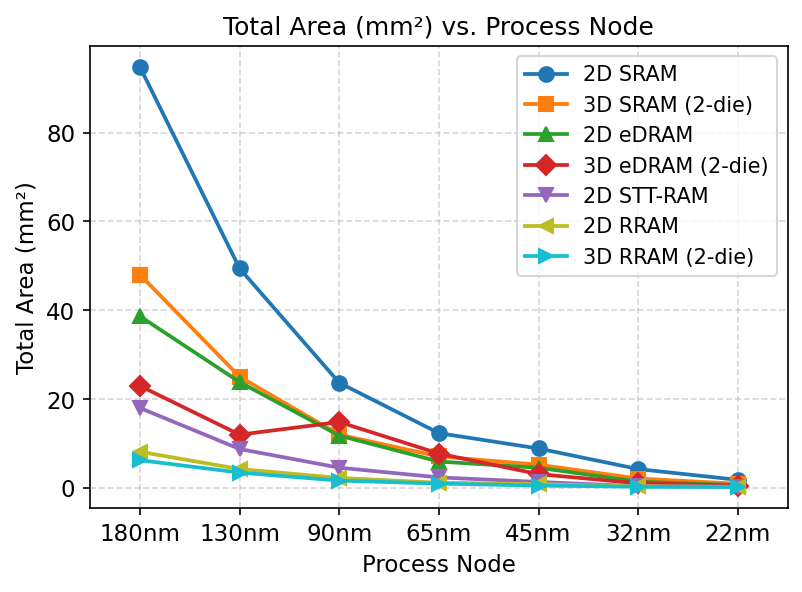
\includegraphics[width=\linewidth]{fig01_total_area_vs_node.png}
        \caption{Total area}
    \end{subfigure}
    \begin{subfigure}[t]{0.32\textwidth}
        \centering
        
\includegraphics[width=\linewidth]{fig02_read_latency_vs_node.png}
        \caption{Read latency}
    \end{subfigure}
    \begin{subfigure}[t]{0.32\textwidth}
        \centering
        
\includegraphics[width=\linewidth]{fig03_write_latency_vs_node.png}
        \caption{Write latency}
    \end{subfigure}

    \vspace{0.15in}

    \begin{subfigure}[t]{0.32\textwidth}
        \centering
        
\includegraphics[width=\linewidth]{fig04_read_energy_vs_node.png}
        \caption{Read dynamic energy}
    \end{subfigure}
    \begin{subfigure}[t]{0.32\textwidth}
        \centering
        
\includegraphics[width=\linewidth]{fig05_write_energy_vs_node.png}
        \caption{Write dynamic energy}
    \end{subfigure}
    \begin{subfigure}[t]{0.32\textwidth}
        \centering
        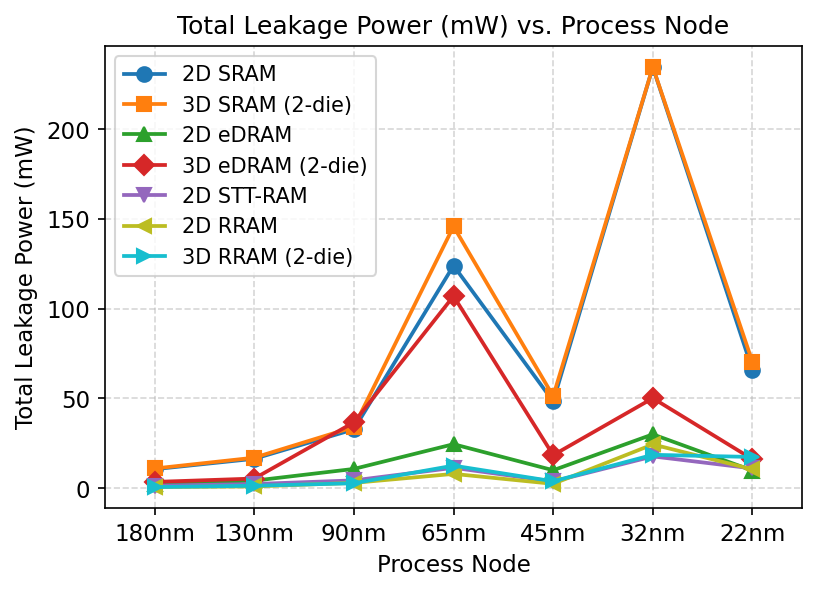
\includegraphics[width=\linewidth]{fig06_leakage_power_vs_node.png}
        \caption{Leakage power}
    \end{subfigure}
    \caption{Process-node scaling trends for different memory technologies.}
    \label{fig:line_results}
\end{figure*}

\subsection{Area Scaling}

The total area decreases clearly from 180 nm to 22 nm for almost all memory technologies. 2D SRAM has the largest area at older nodes because of its 6T bitcell structure. eDRAM and RRAM show better density due to more compact cell structures. 3D versions generally reduce the effective planar footprint, although the benefit depends on TSV overhead and internal memory organization.

At advanced nodes, the difference between technologies becomes smaller in absolute value, but 3D eDRAM and RRAM-based technologies remain highly area-efficient. This confirms that area scaling is driven by both process-node shrink and memory-cell topology.

\subsection{Latency Trends}

Read and write latency show more complex behavior than area. SRAM has high latency at older nodes because the large array footprint increases global interconnect and H-tree delay. 3D SRAM reduces this latency by shrinking the effective horizontal footprint. eDRAM, especially 3D eDRAM, shows strong latency performance at advanced nodes.

For non-volatile memories such as RRAM and STT-RAM, write latency remains relatively high because it is more strongly related to device-level programming behavior. Therefore, their write-latency trend should be interpreted as technology-model dependent rather than purely CMOS-scaling dependent.

\subsection{Dynamic Energy Trends}

Read dynamic energy generally decreases with node scaling because smaller technology nodes reduce capacitance and supply voltage. Write dynamic energy is more non-monotonic. It can be interpreted using
\begin{equation}
E_{\mathrm{write}} = C_{\mathrm{switched}} V_{DD}^{2} \alpha ,
\label{eq:energy}
\end{equation}
where $C_{\mathrm{switched}}$ is the switched capacitance, $V_{DD}$ is the supply voltage, and $\alpha$ is the activity factor.

Although process scaling tends to reduce $V_{DD}$ and capacitance, DESTINY may choose a more parallel organization to reduce delay. This can activate more mats, subarrays, or bitlines, increasing $C_{\mathrm{switched}}$ and producing non-monotonic write energy.

\subsection{Leakage Power}

Leakage power is strongly affected by the memory cell structure. SRAM generally has higher leakage due to its 6T cell. eDRAM has lower leakage because its 1T-1C cell has fewer transistors per bit. However, 3D designs may introduce additional leakage due to TSV drivers, receivers, and extra peripheral circuitry.

The leakage spike observed for SRAM at 32 nm is likely caused by the optimizer selecting a high-parallelism structure under WriteEDP optimization. This increases the number of active or standby-biased transistors and therefore increases total leakage.

\section{Heatmap-Based Technology Comparison}

The heatmaps in Fig.~\ref{fig:heatmaps} provide a compact view of technology-node tradeoffs. Green regions indicate better values, while red regions indicate worse values. This format makes it easier to compare a large number of memory technologies across multiple process nodes.

\begin{figure*}[t]
    \centering
    \begin{subfigure}[t]{0.32\textwidth}
        \centering
        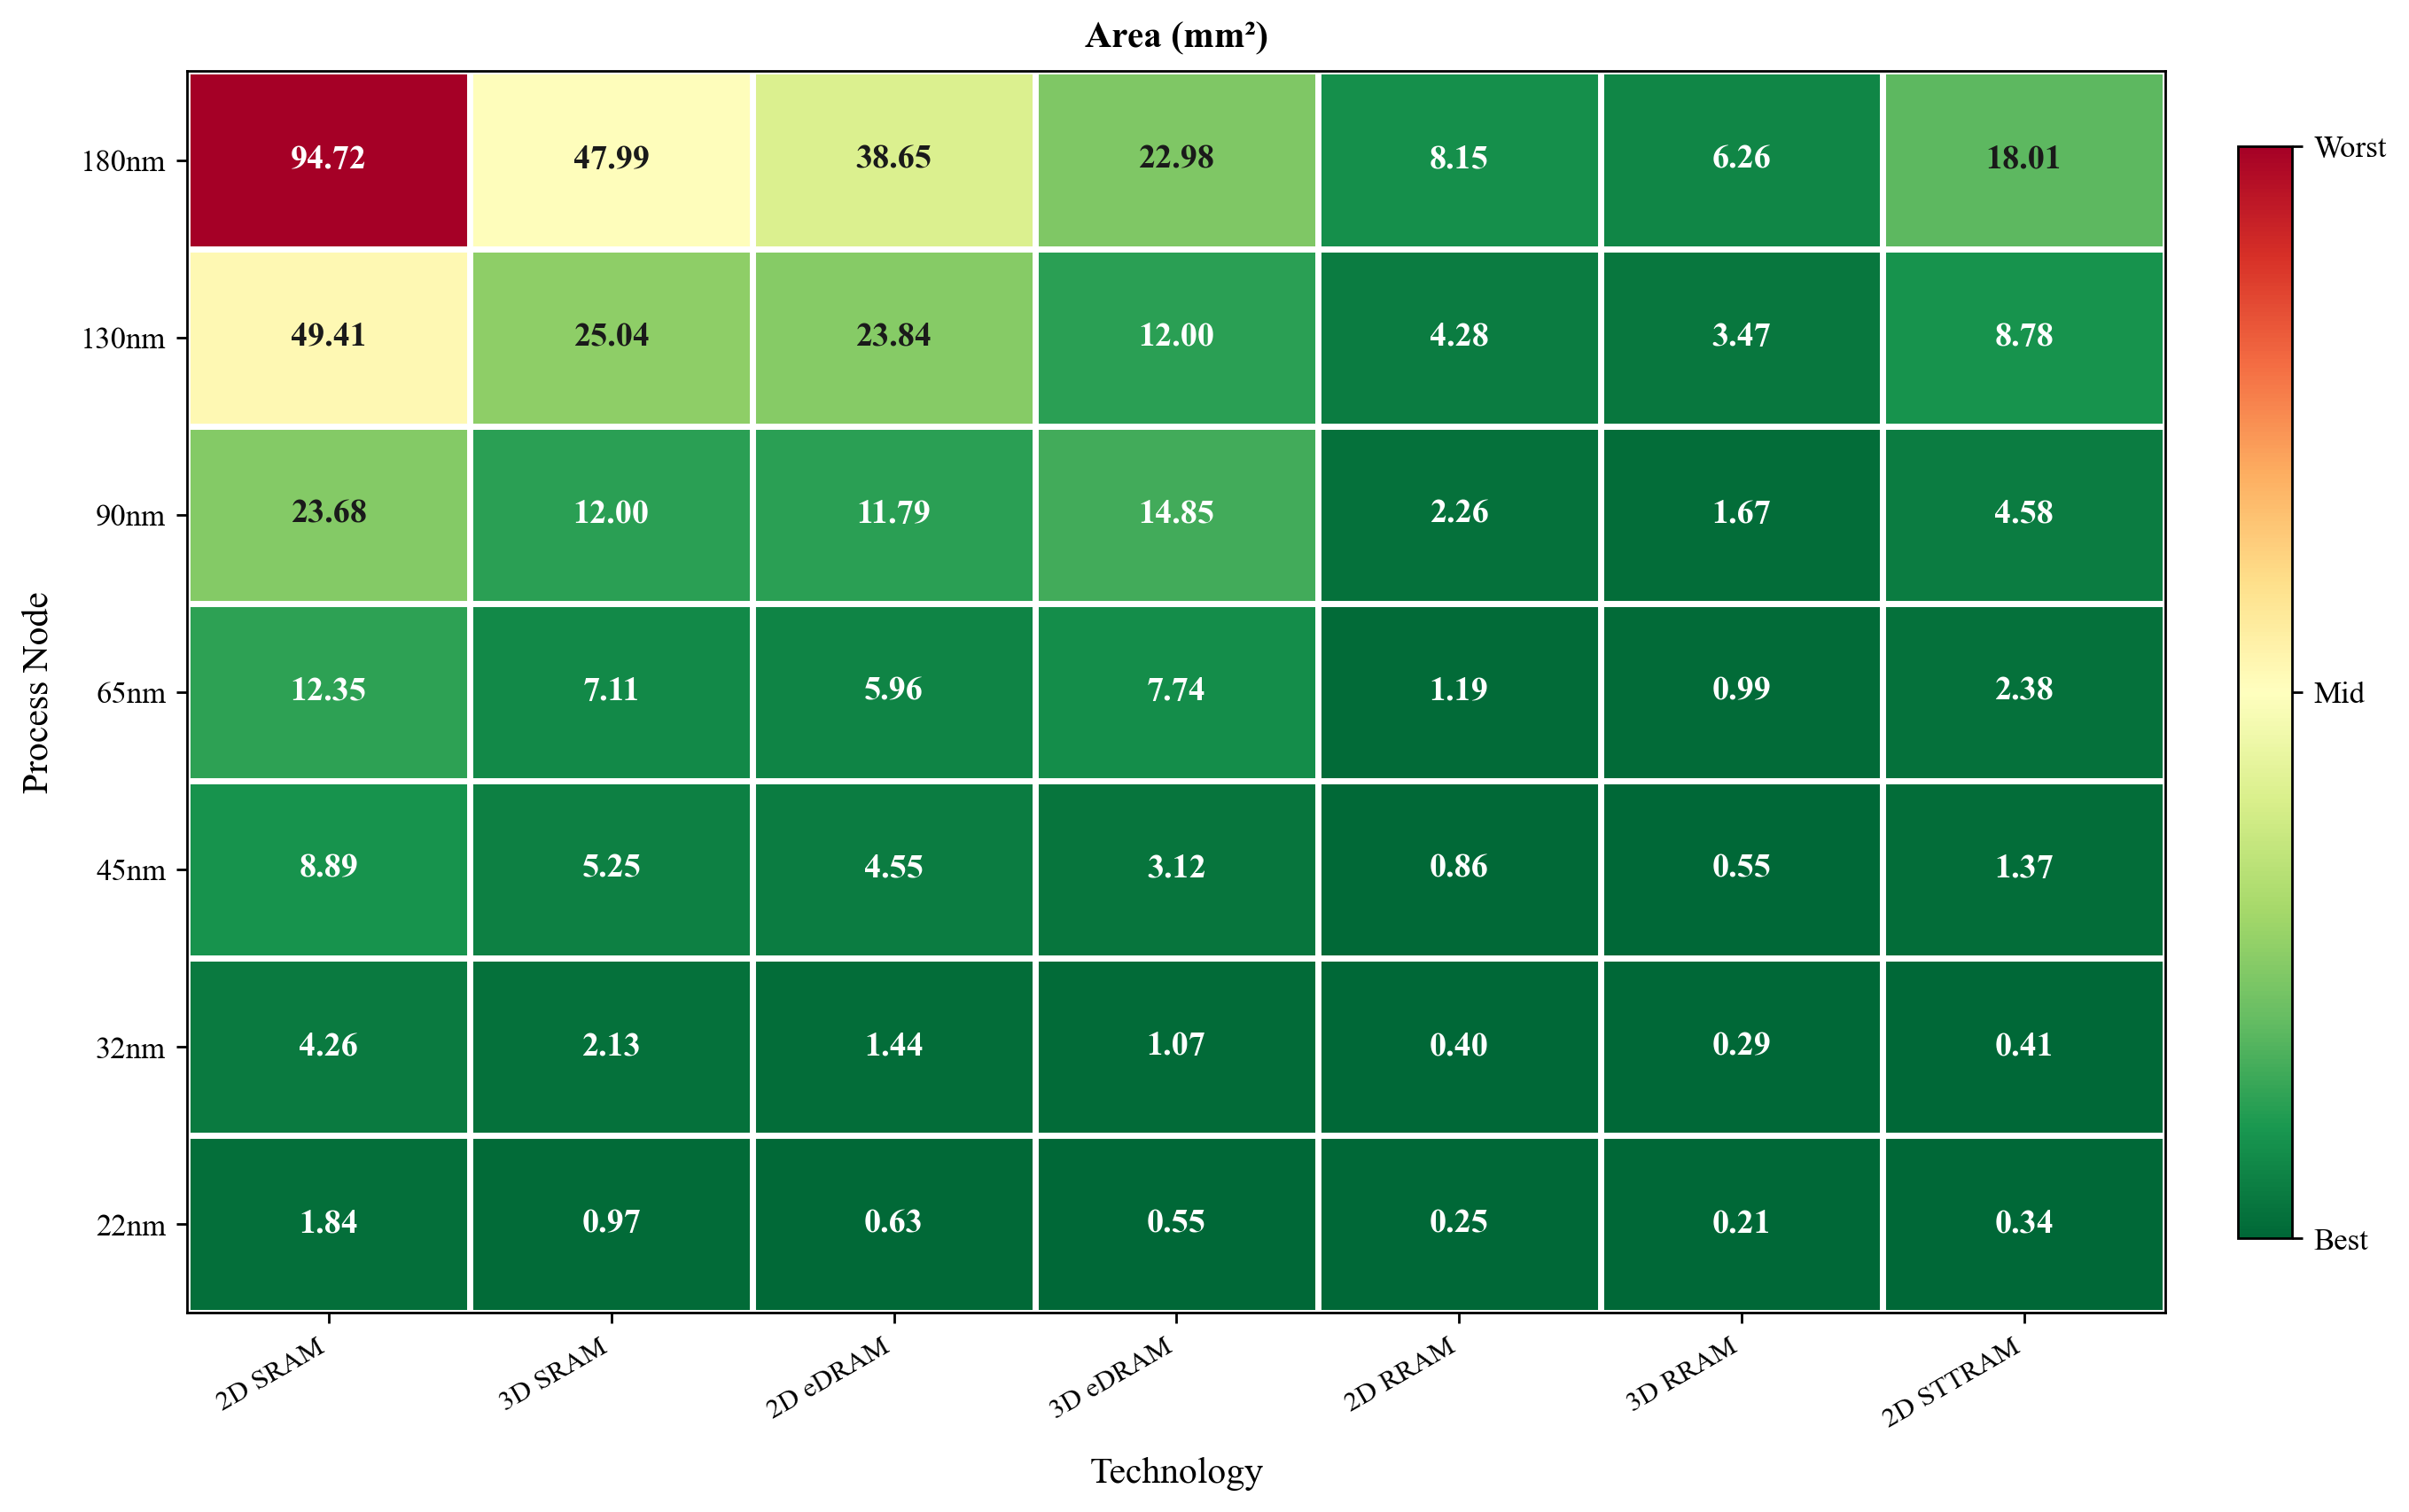
\includegraphics[width=\linewidth]{heatmap_total_area.png}
        \caption{Area}
    \end{subfigure}
    \begin{subfigure}[t]{0.32\textwidth}
        \centering
        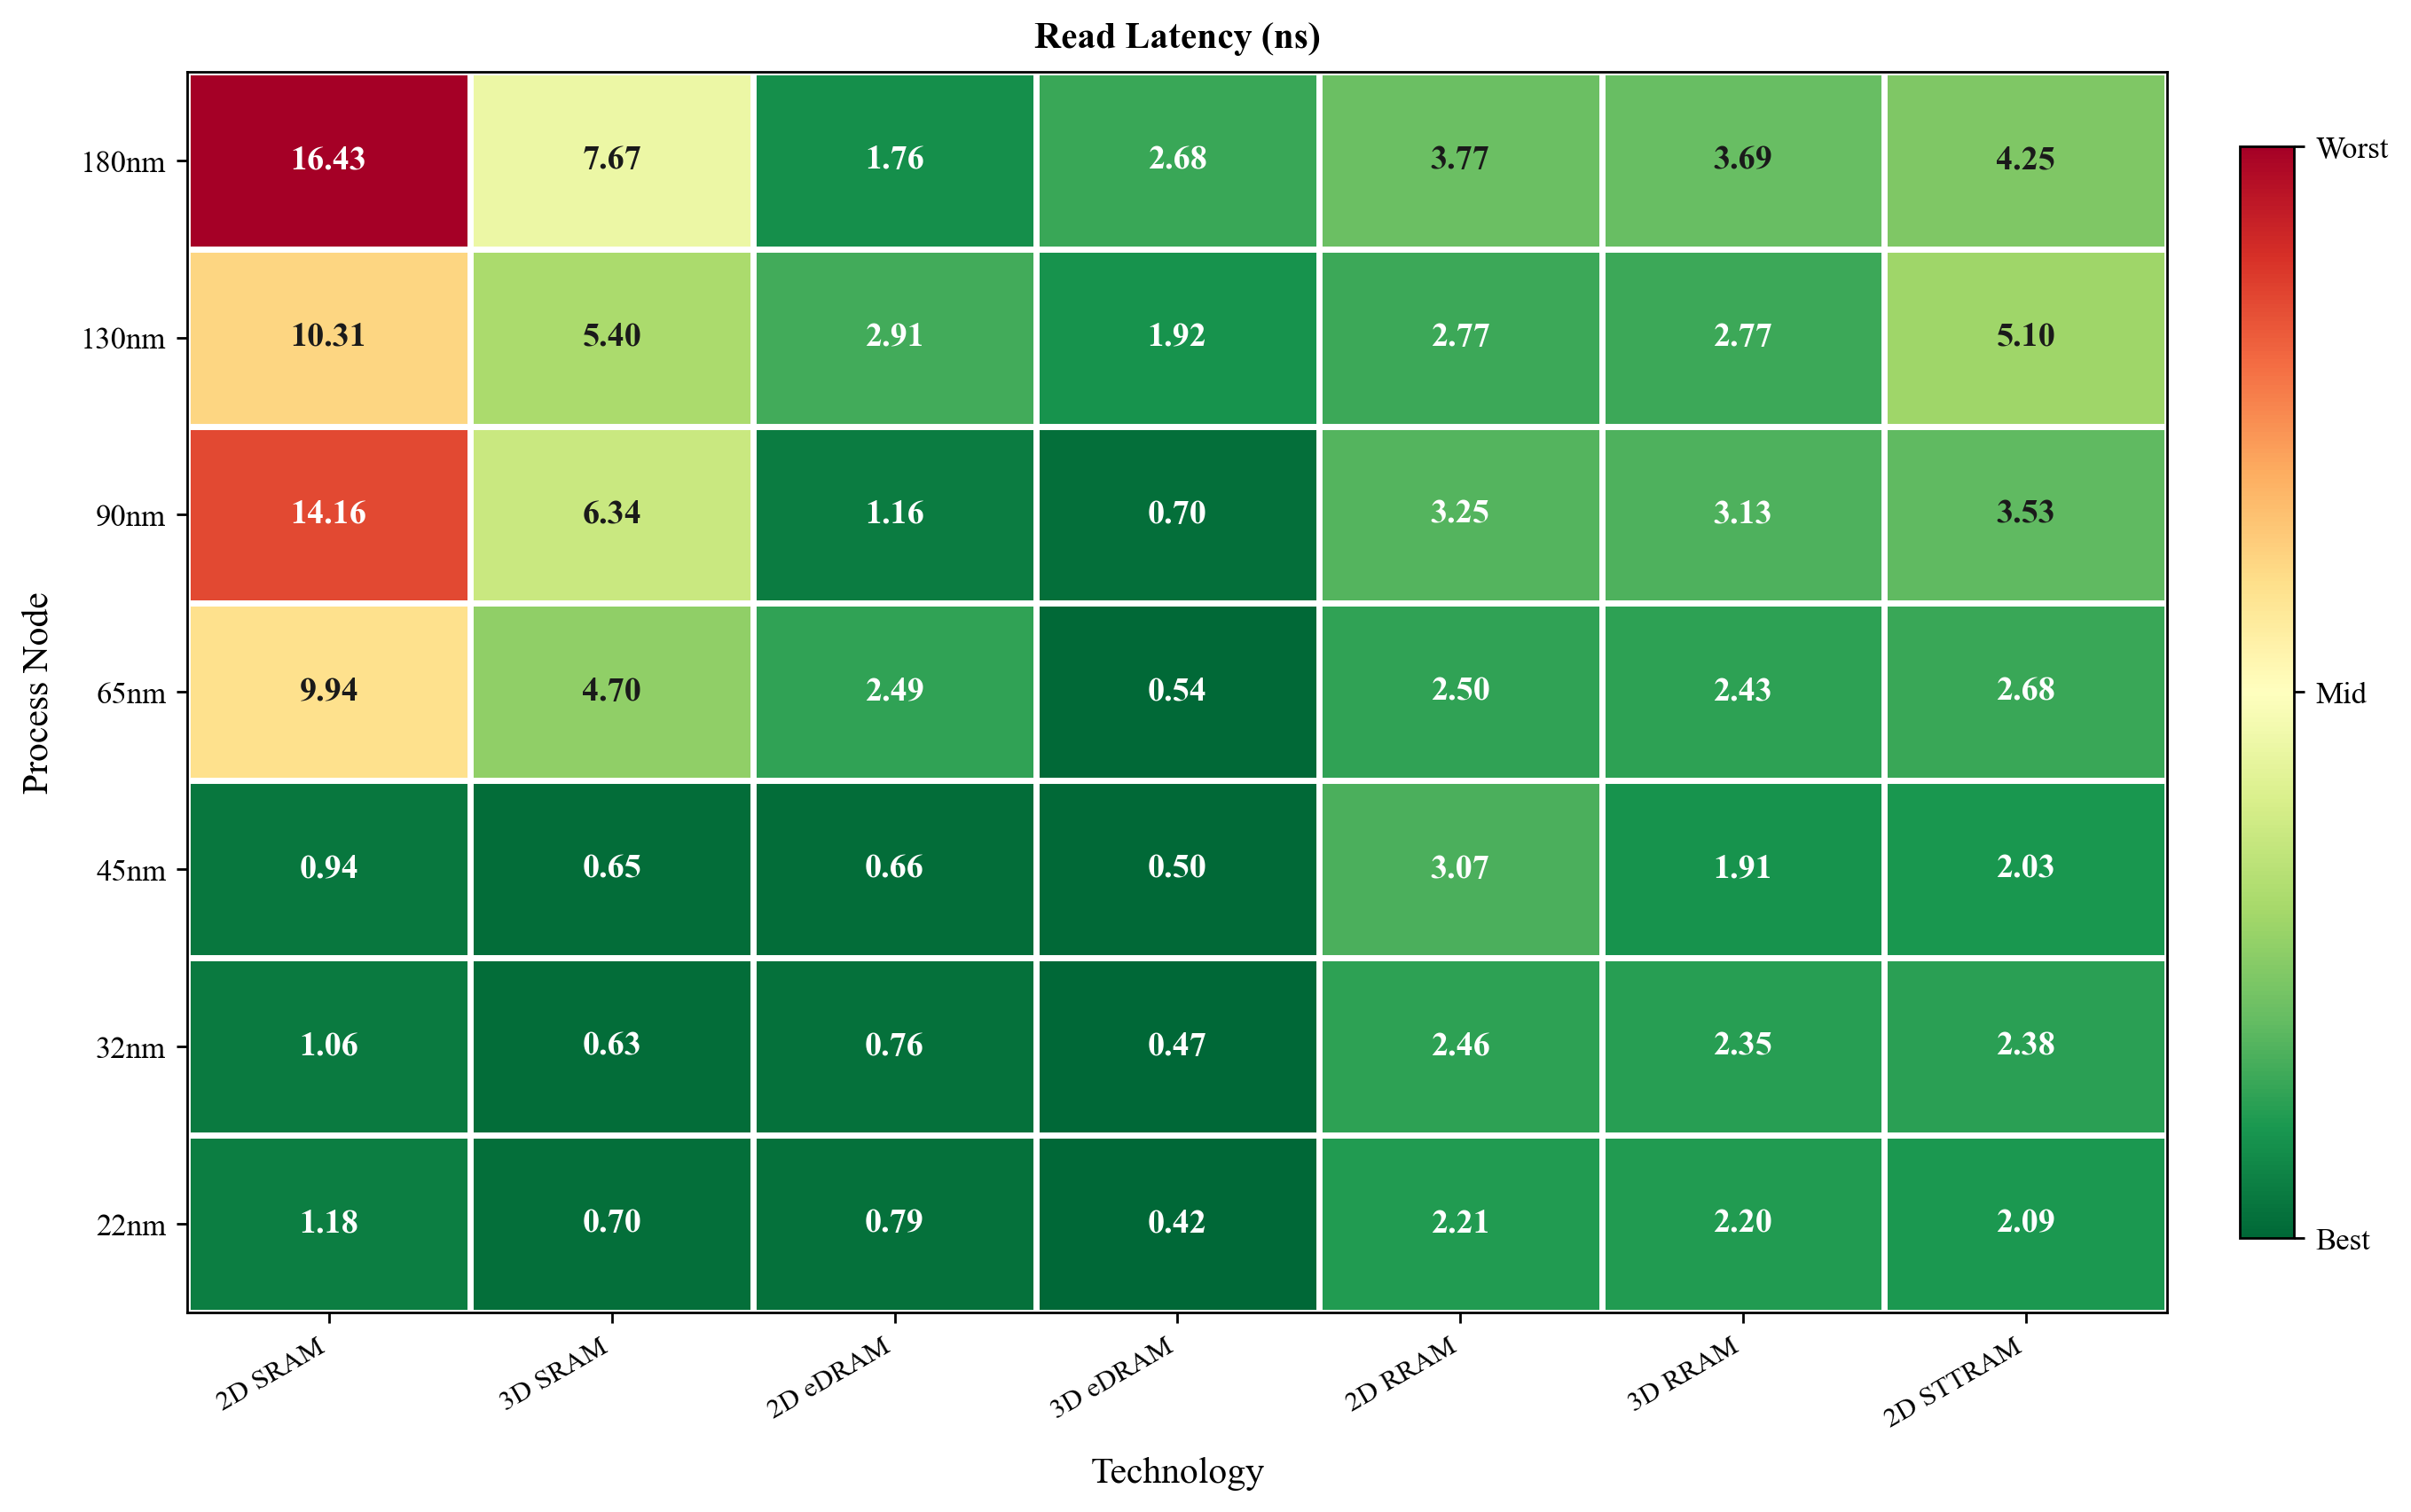
\includegraphics[width=\linewidth]{heatmap_read_latency.png}
        \caption{Read latency}
    \end{subfigure}
    \begin{subfigure}[t]{0.32\textwidth}
        \centering
        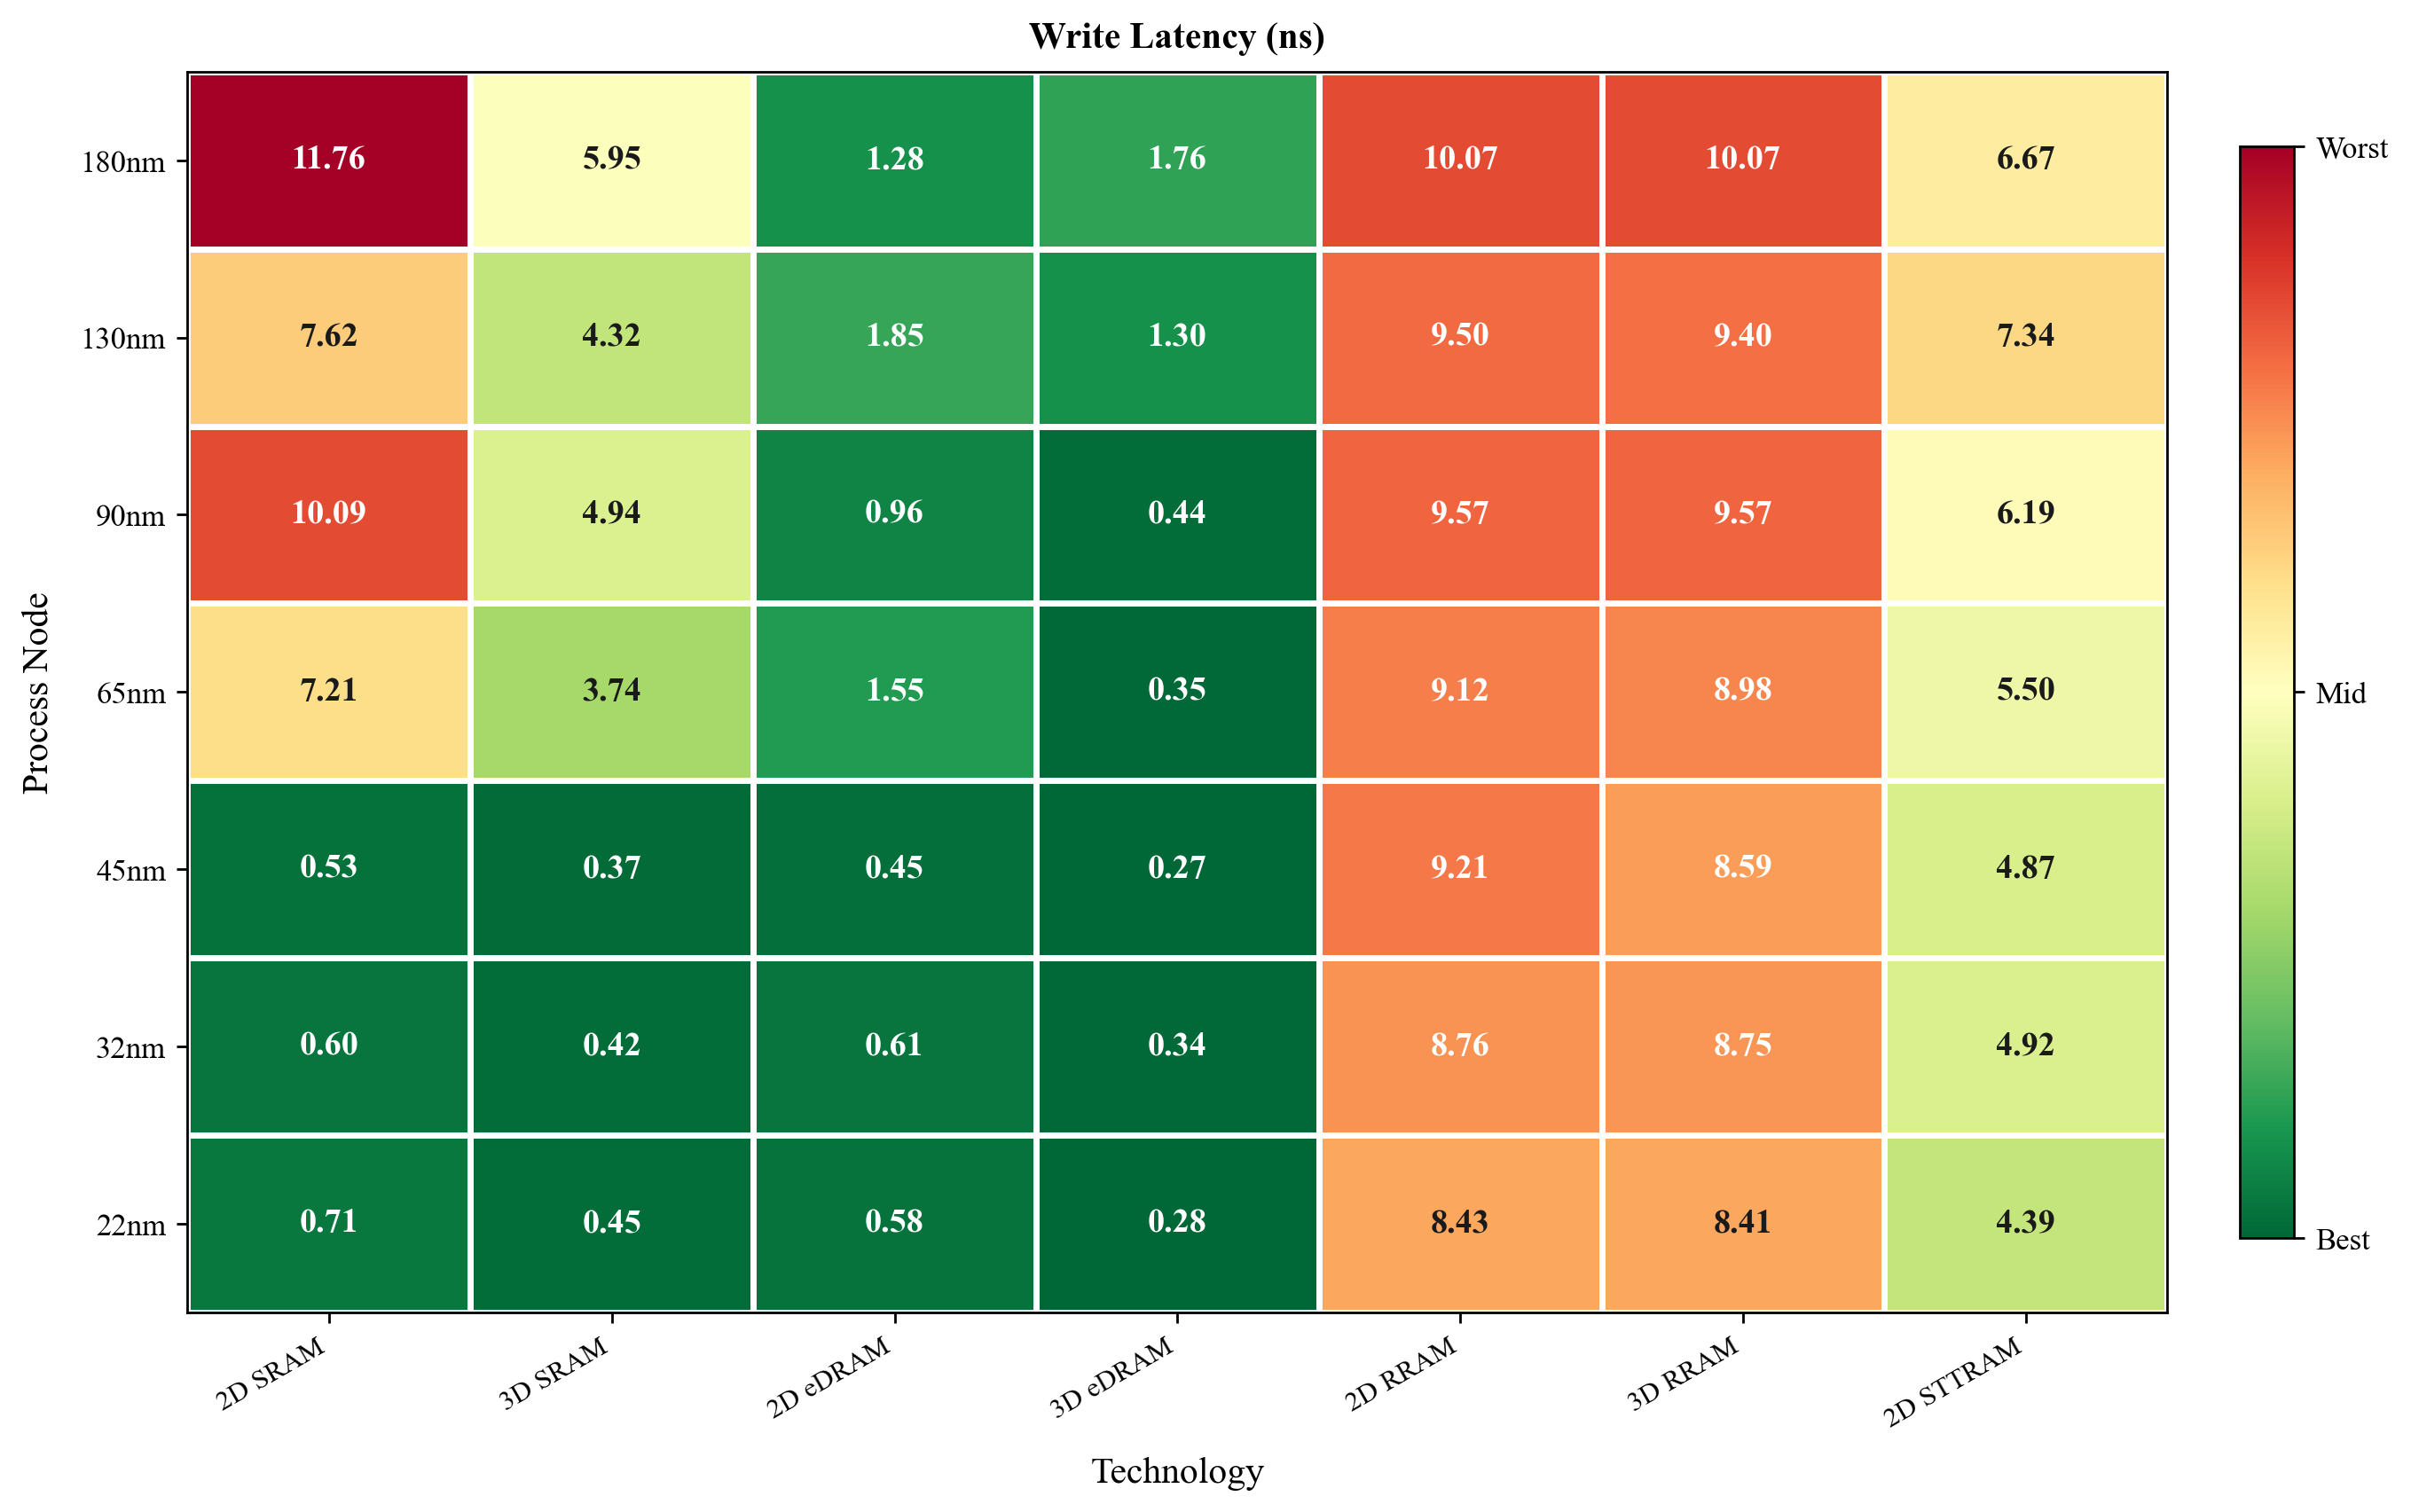
\includegraphics[width=\linewidth]{heatmap_write_latency.png}
        \caption{Write latency}
    \end{subfigure}

    \vspace{0.15in}

    \begin{subfigure}[t]{0.32\textwidth}
        \centering
        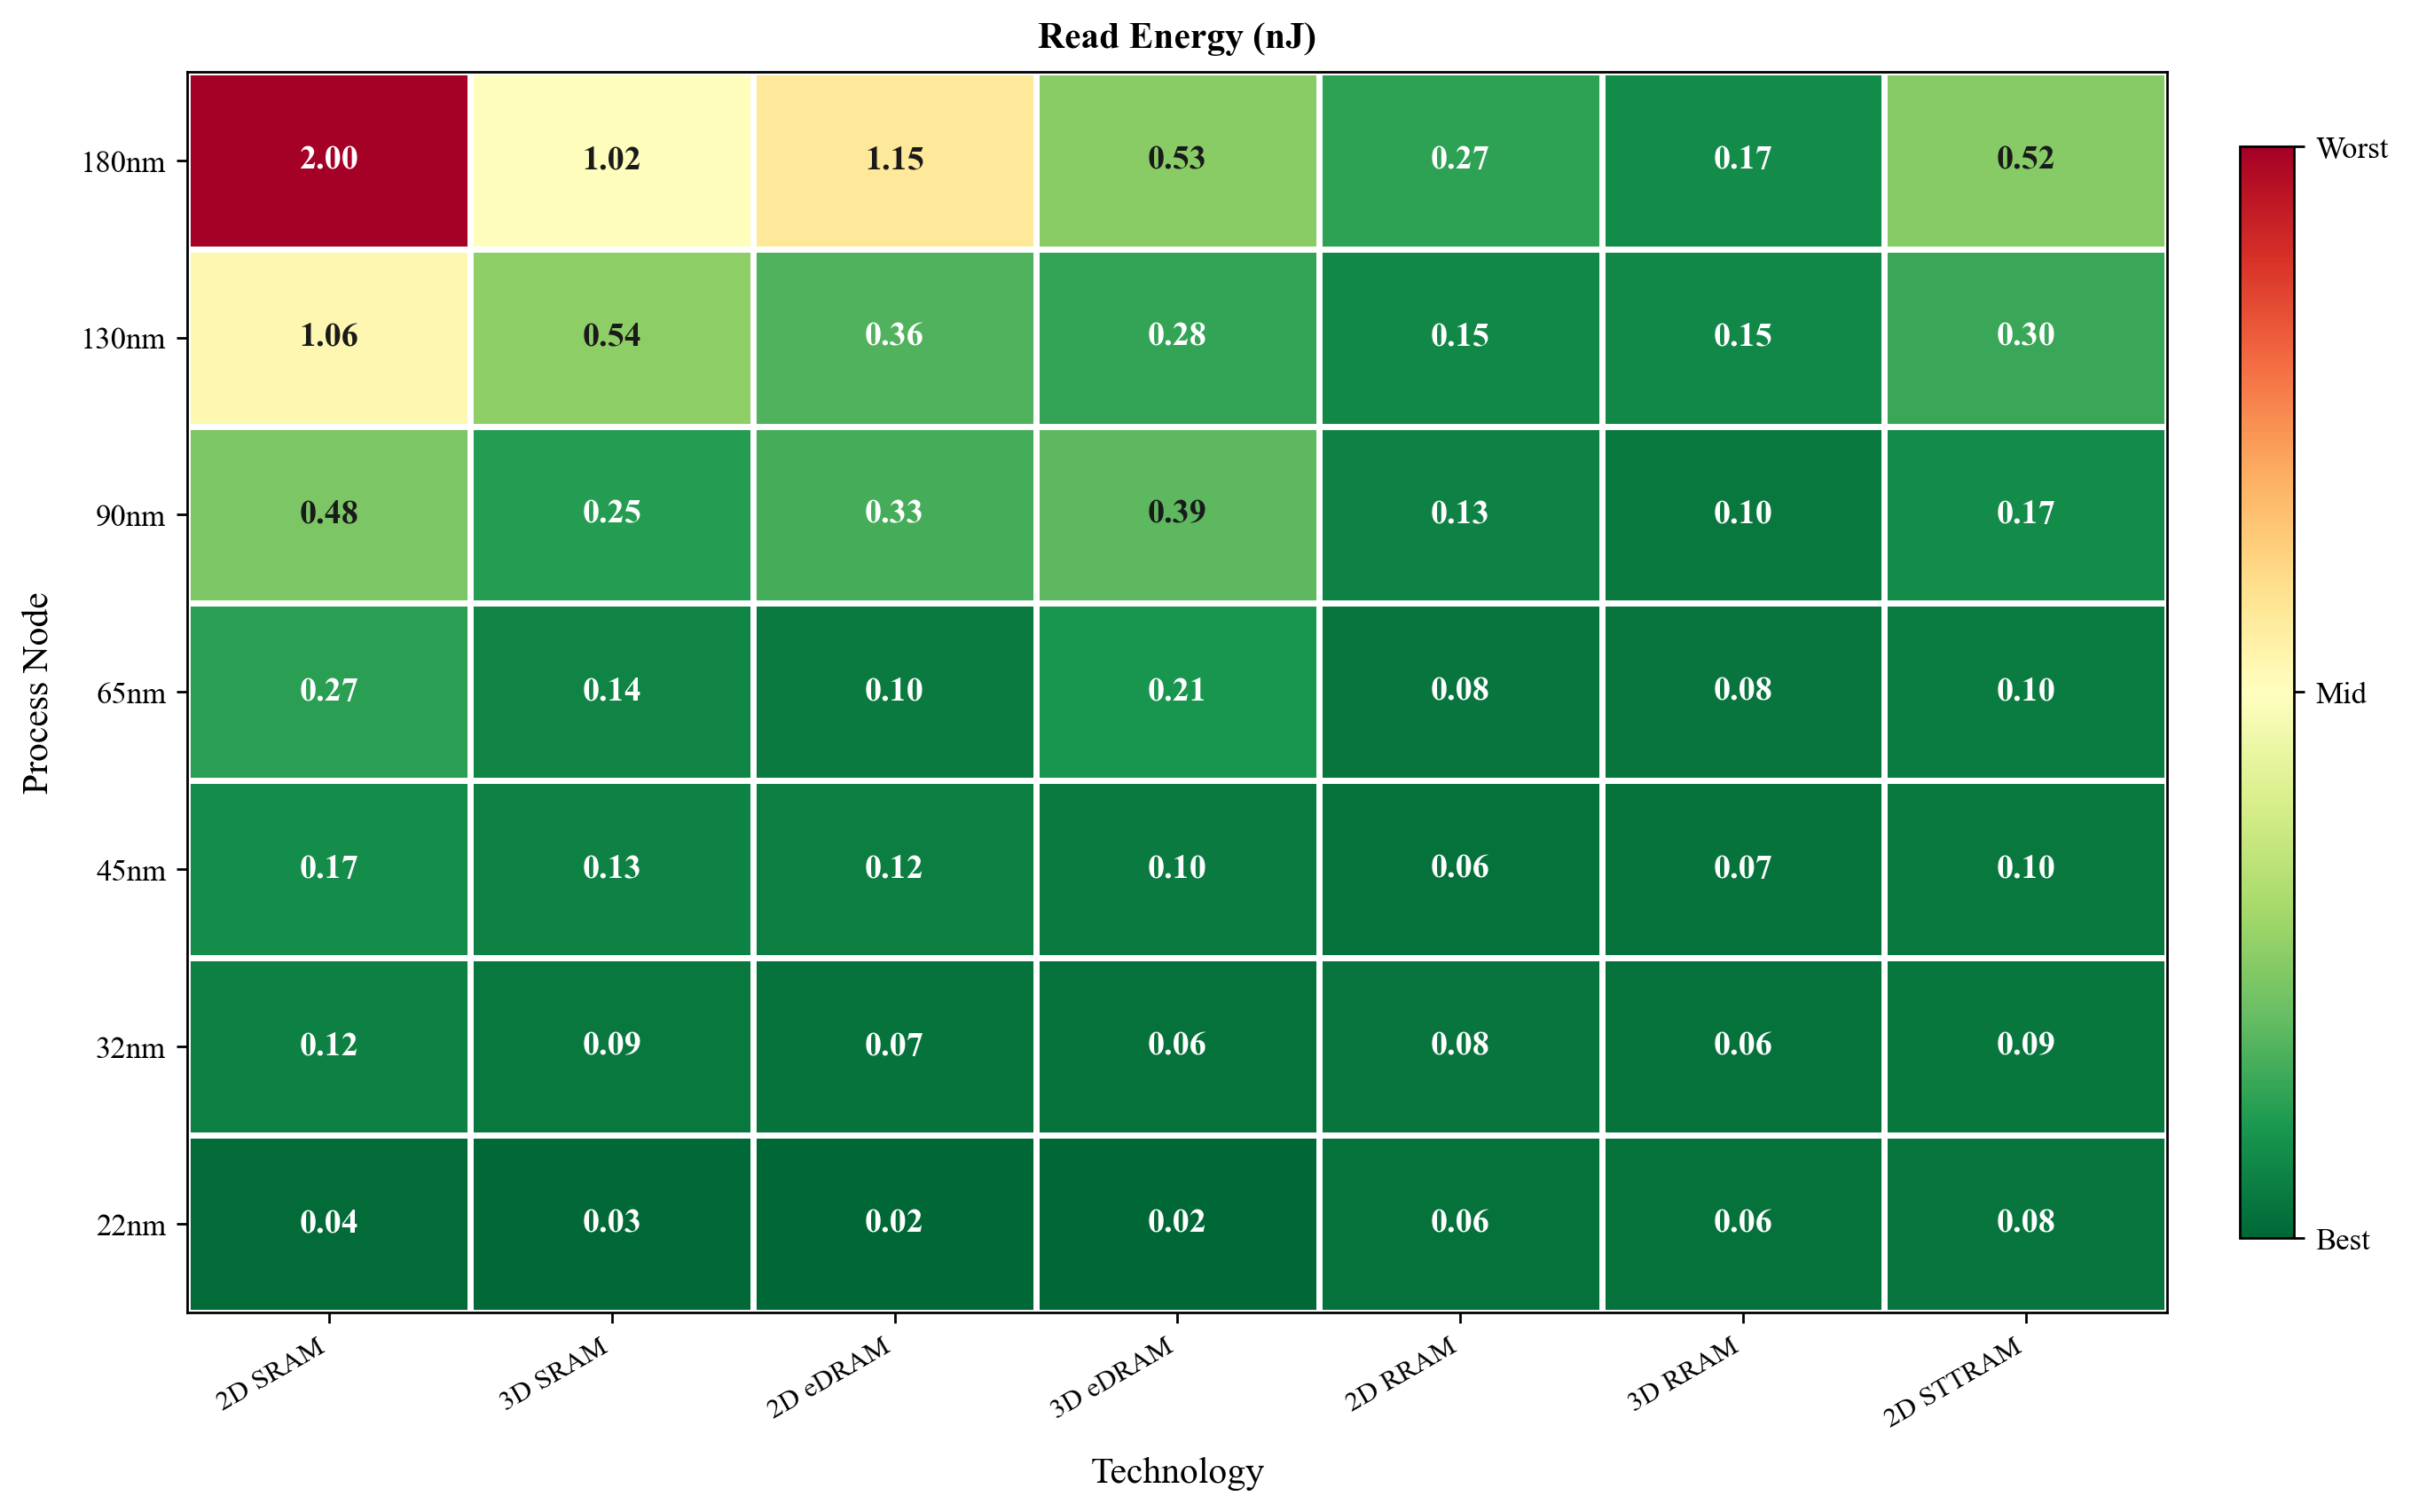
\includegraphics[width=\linewidth]{heatmap_read_energy.png}
        \caption{Read energy}
    \end{subfigure}
    \begin{subfigure}[t]{0.32\textwidth}
        \centering
        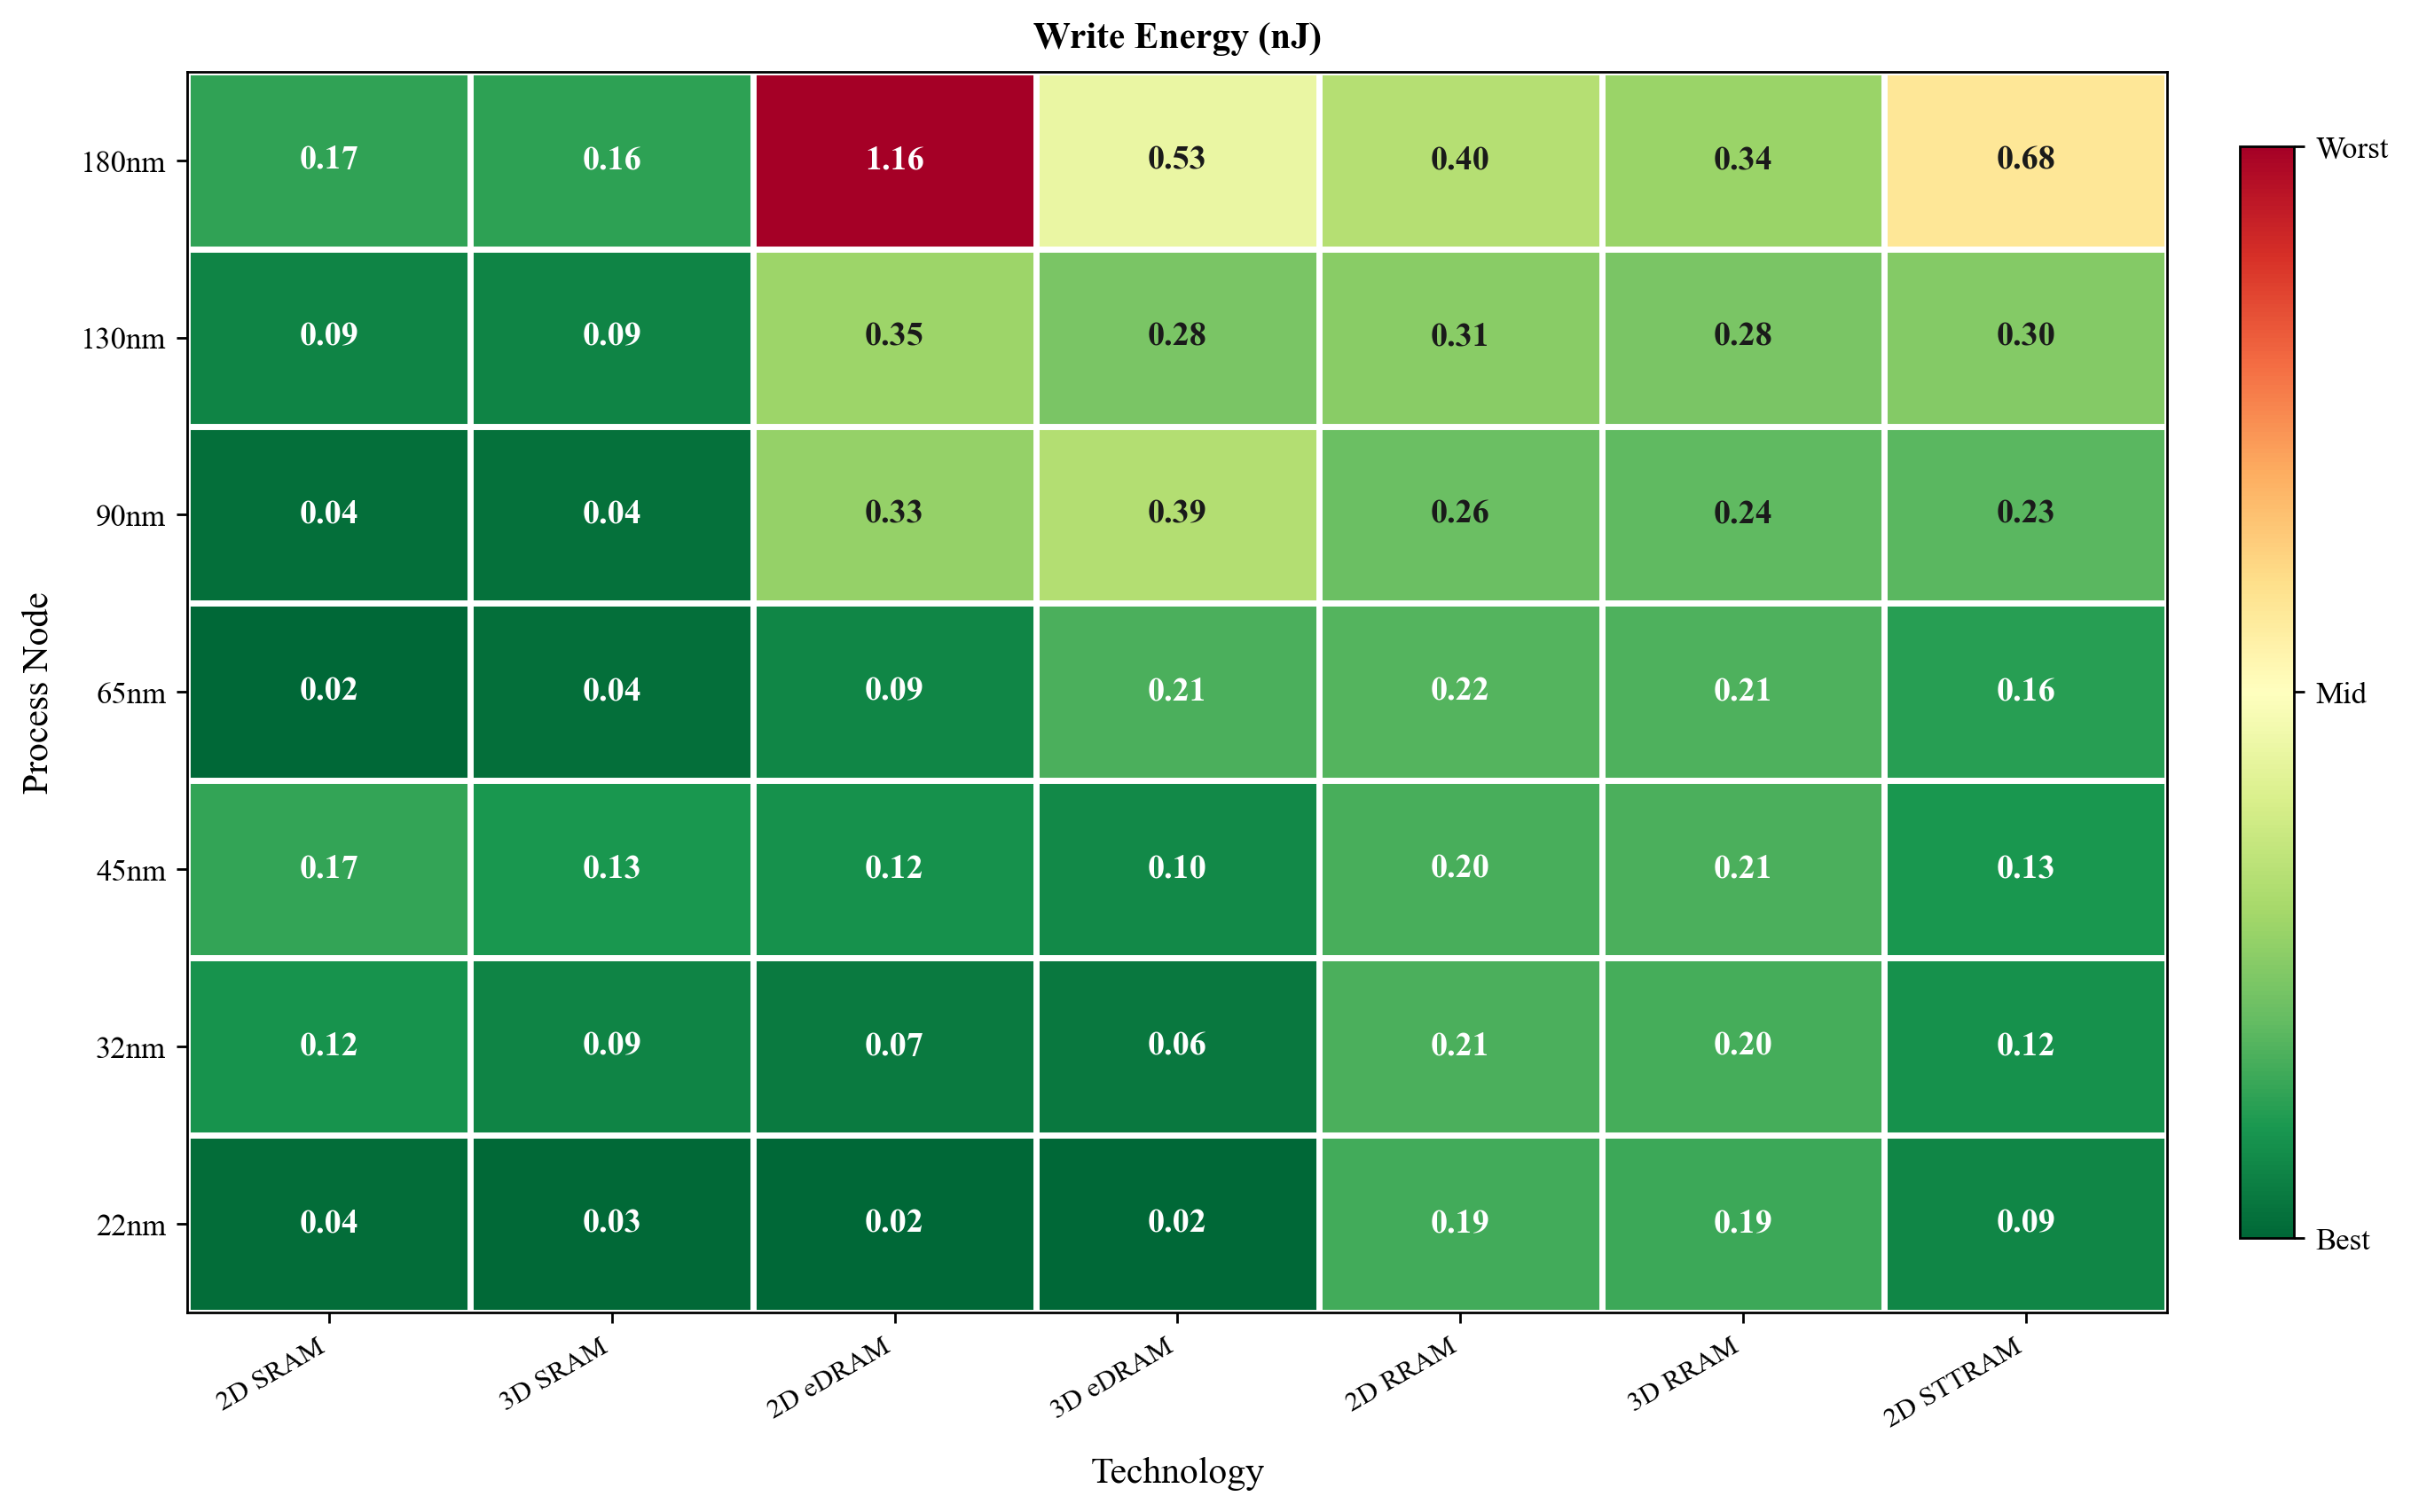
\includegraphics[width=\linewidth]{heatmap_write_energy.png}
        \caption{Write energy}
    \end{subfigure}
    \begin{subfigure}[t]{0.32\textwidth}
        \centering
        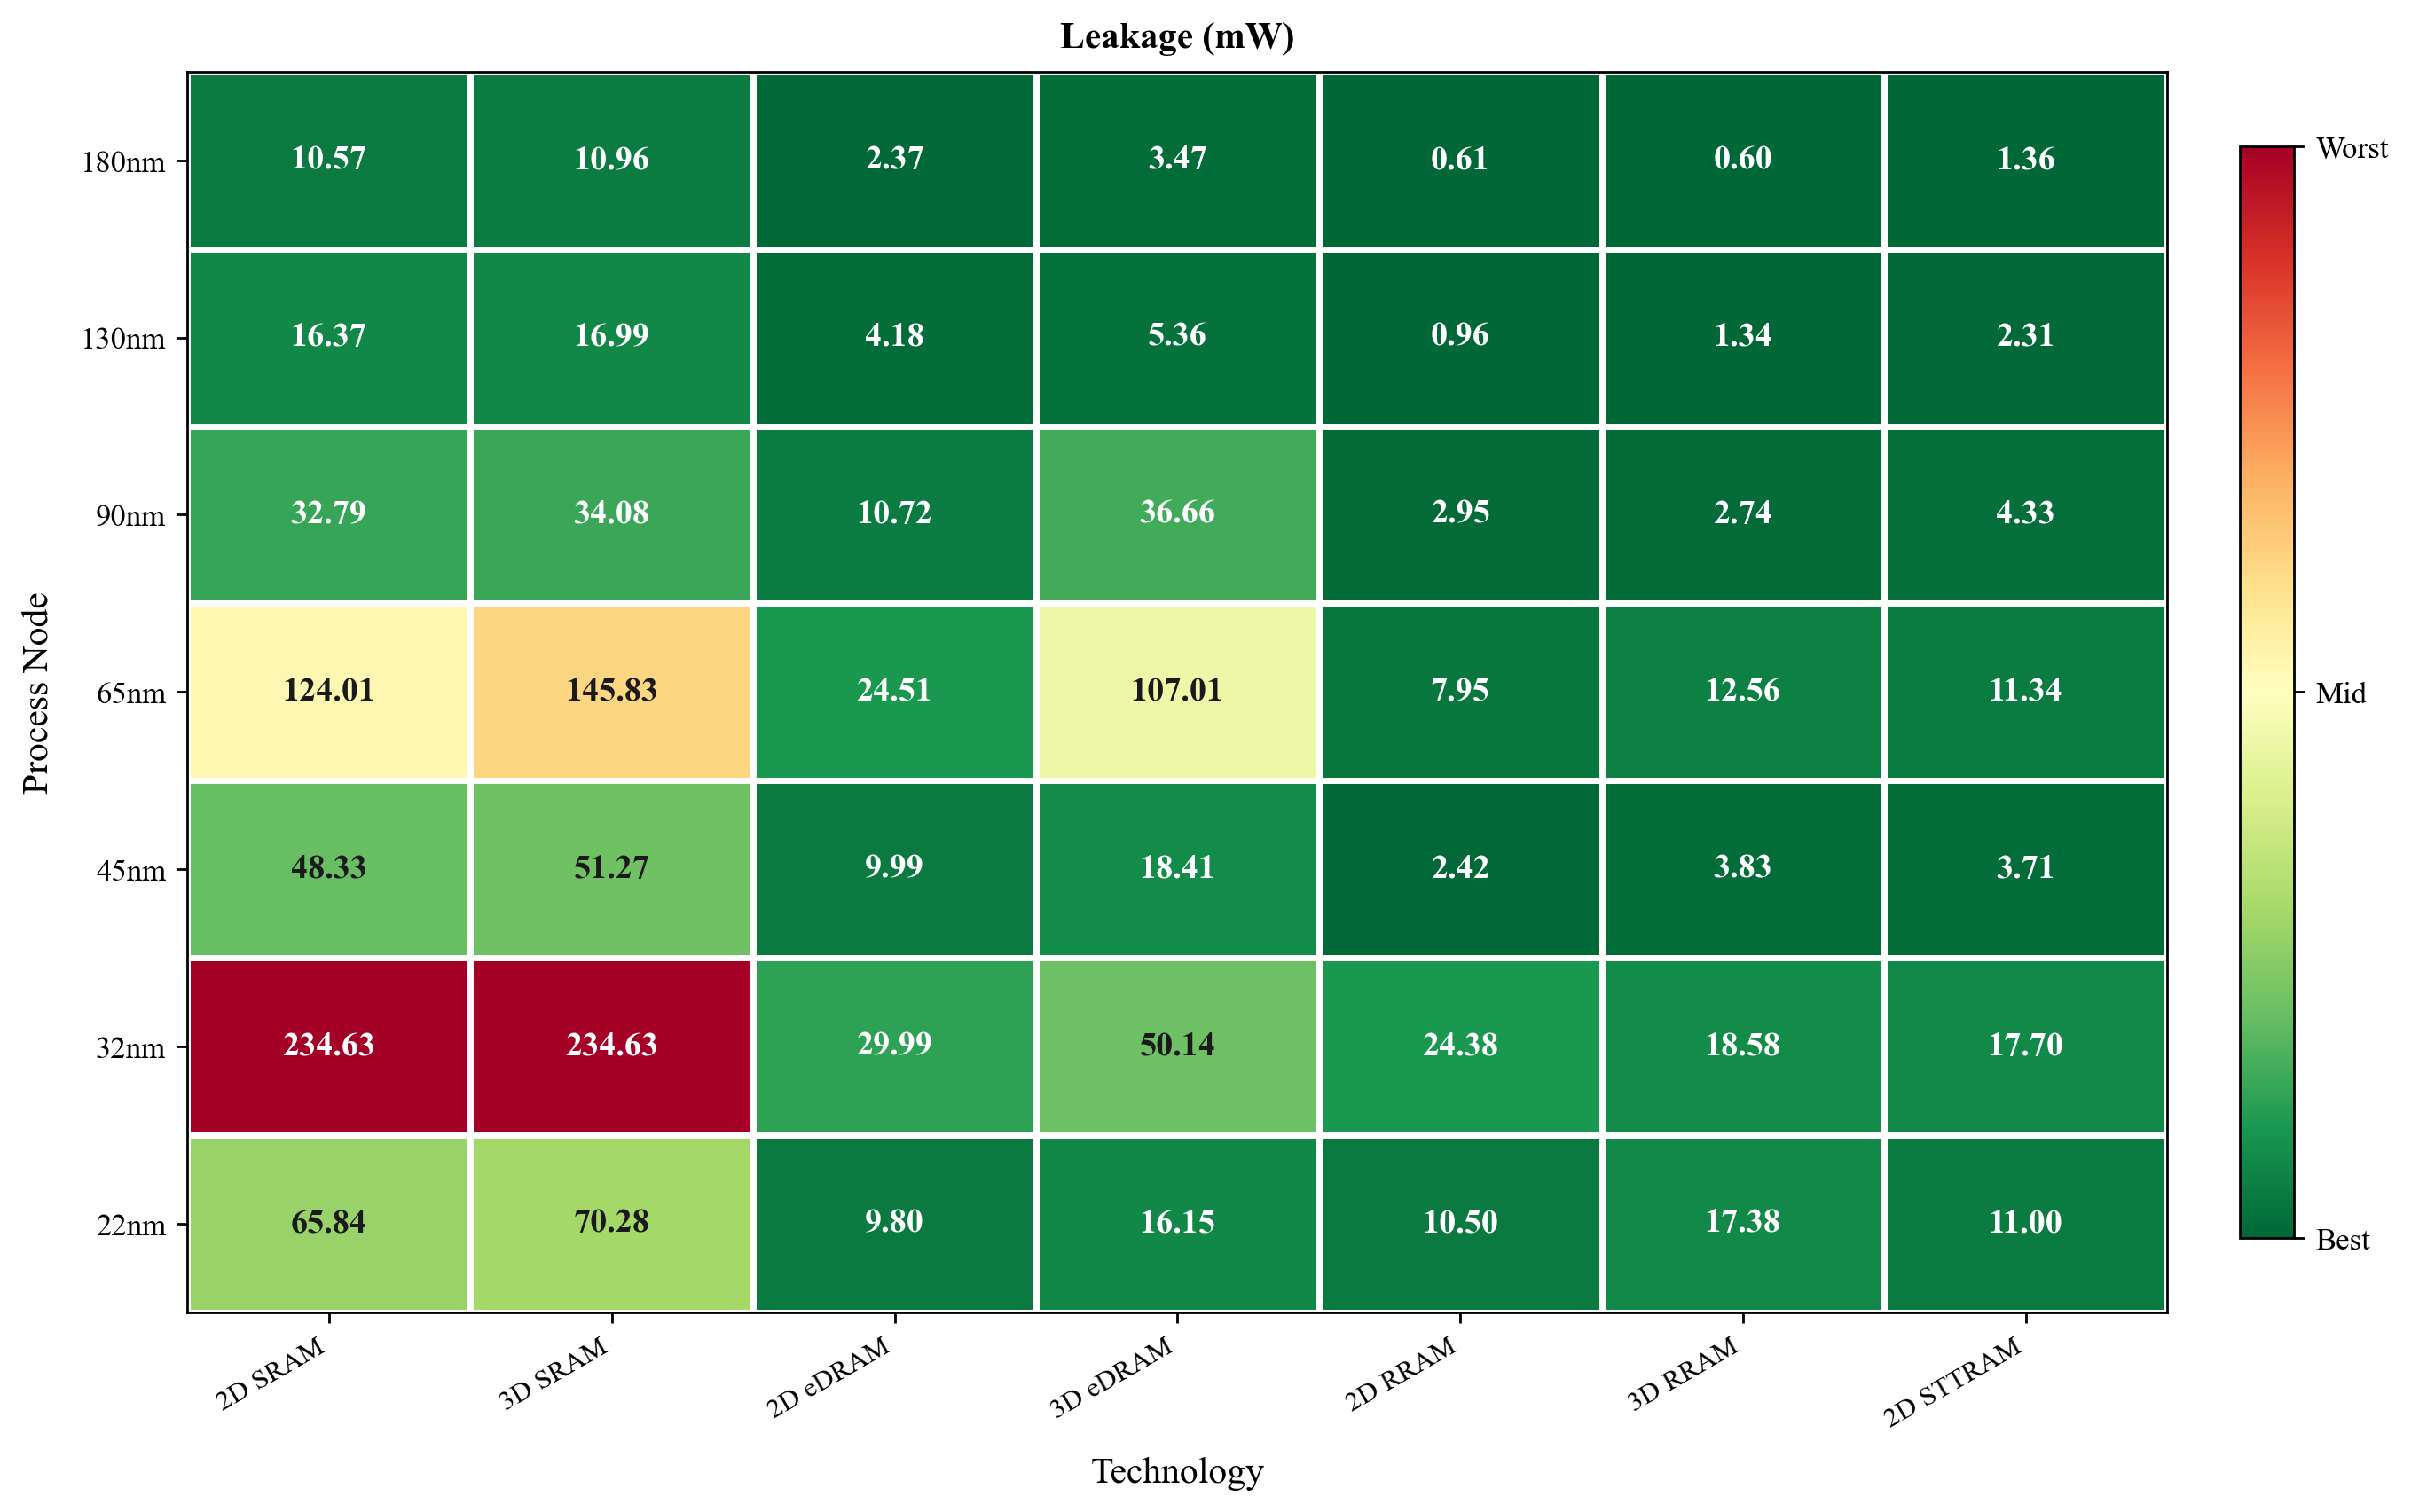
\includegraphics[width=\linewidth]{heatmap_leakage_power.png}
        \caption{Leakage power}
    \end{subfigure}
    \caption{Heatmap comparison of memory technologies across process nodes.}
    \label{fig:heatmaps}
\end{figure*}

The area heatmap shows that SRAM is the least area-efficient at older nodes, while RRAM and eDRAM achieve much smaller footprints. The read-latency heatmap shows that 3D eDRAM is one of the strongest options at advanced nodes. The write-latency heatmap highlights the disadvantage of RRAM and STT-RAM for write-dominated workloads. The leakage heatmap further shows that SRAM has high leakage at several nodes, while eDRAM and RRAM generally provide lower leakage.

Overall, the heatmaps confirm that memory technology selection depends strongly on the target metric. A technology that is strong in area may not be strong in write latency, and a technology with low leakage may have higher write cost.

\section{Layer Scaling and EDP Improvement}

Fig.~\ref{fig:layer_scaling} shows how stacked-die count affects area improvement, read EDP improvement, and write EDP improvement relative to the 1-layer baseline.

\begin{figure*}[t]
    \centering
    \begin{subfigure}[t]{0.32\textwidth}
        \centering
        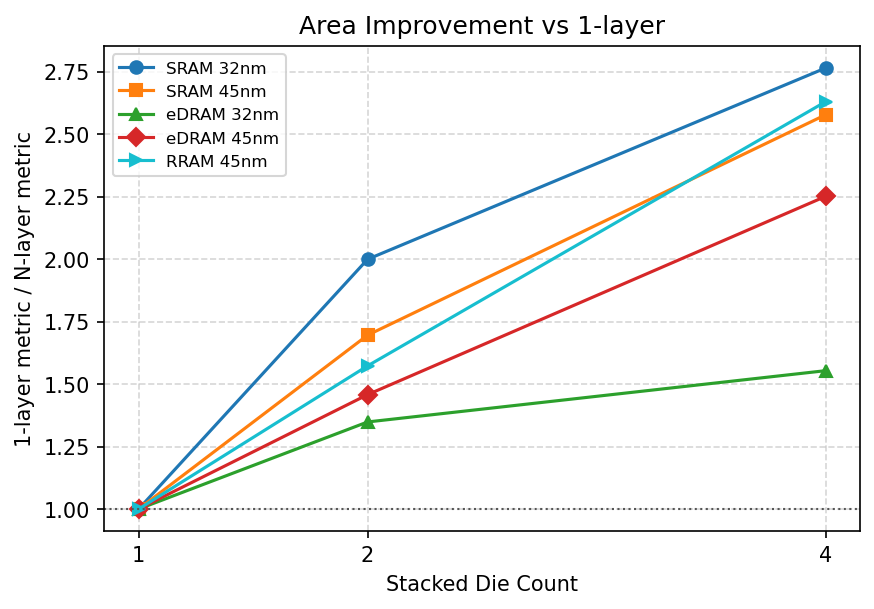
\includegraphics[width=\linewidth]{fig20_layer_area_improvement.png}
        \caption{Area improvement}
    \end{subfigure}
    \begin{subfigure}[t]{0.32\textwidth}
        \centering
        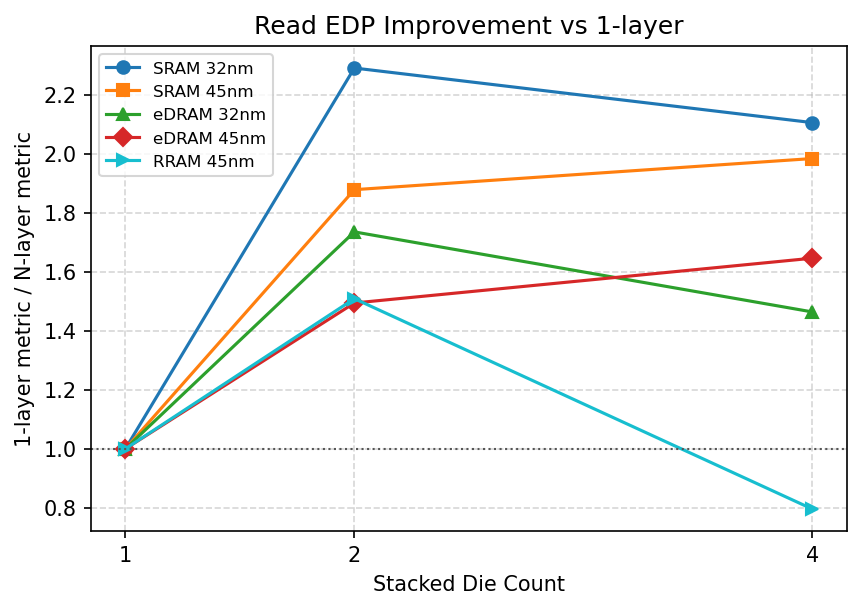
\includegraphics[width=\linewidth]{fig21_layer_read_edp_improvement.png}
        \caption{Read EDP improvement}
    \end{subfigure}
    \begin{subfigure}[t]{0.32\textwidth}
        \centering
        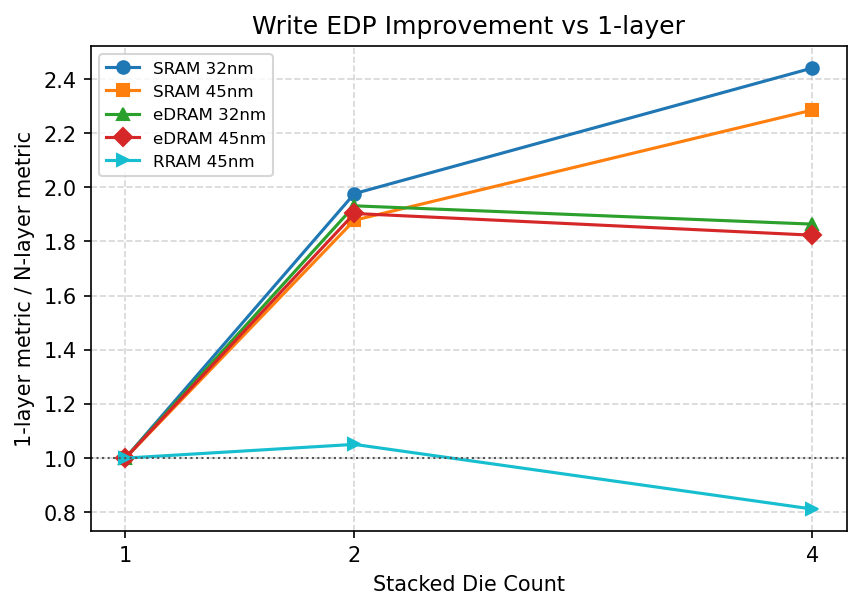
\includegraphics[width=\linewidth]{fig22_layer_write_edp_improvement.png}
        \caption{Write EDP improvement}
    \end{subfigure}
    \caption{Stacked-die improvement relative to the 1-layer baseline.}
    \label{fig:layer_scaling}
\end{figure*}

The area improvement generally increases as the stacked-die count increases. SRAM benefits strongly from stacking because its original 2D footprint is large. eDRAM also benefits from stacking, but the improvement is more limited because eDRAM already has a compact cell structure.

Read EDP improvement is not always monotonic. For example, some technologies improve from 1-layer to 2-layer but show reduced benefit at 4-layer. This suggests that increasing the number of dies does not automatically improve performance. The improvement from shorter horizontal interconnects can be offset by TSV overhead, routing complexity, and optimizer-selected organization changes.

Write EDP improvement shows a similar trend. SRAM and eDRAM benefit from stacking, while RRAM can show weaker or even negative improvement at higher layer count. This indicates that if write behavior is dominated by cell-level programming physics, additional stacking may not significantly improve write-side efficiency.

\section{PPA Tradeoff Visualization}

\subsection{Area vs. Read Latency Scatter Plot}

Fig.~\ref{fig:ppa_scatter} shows the PPA tradeoff space using area and read latency. The curves run from older nodes to advanced nodes, and the marker size indicates process node.

\begin{figure*}[t]
    \centering
    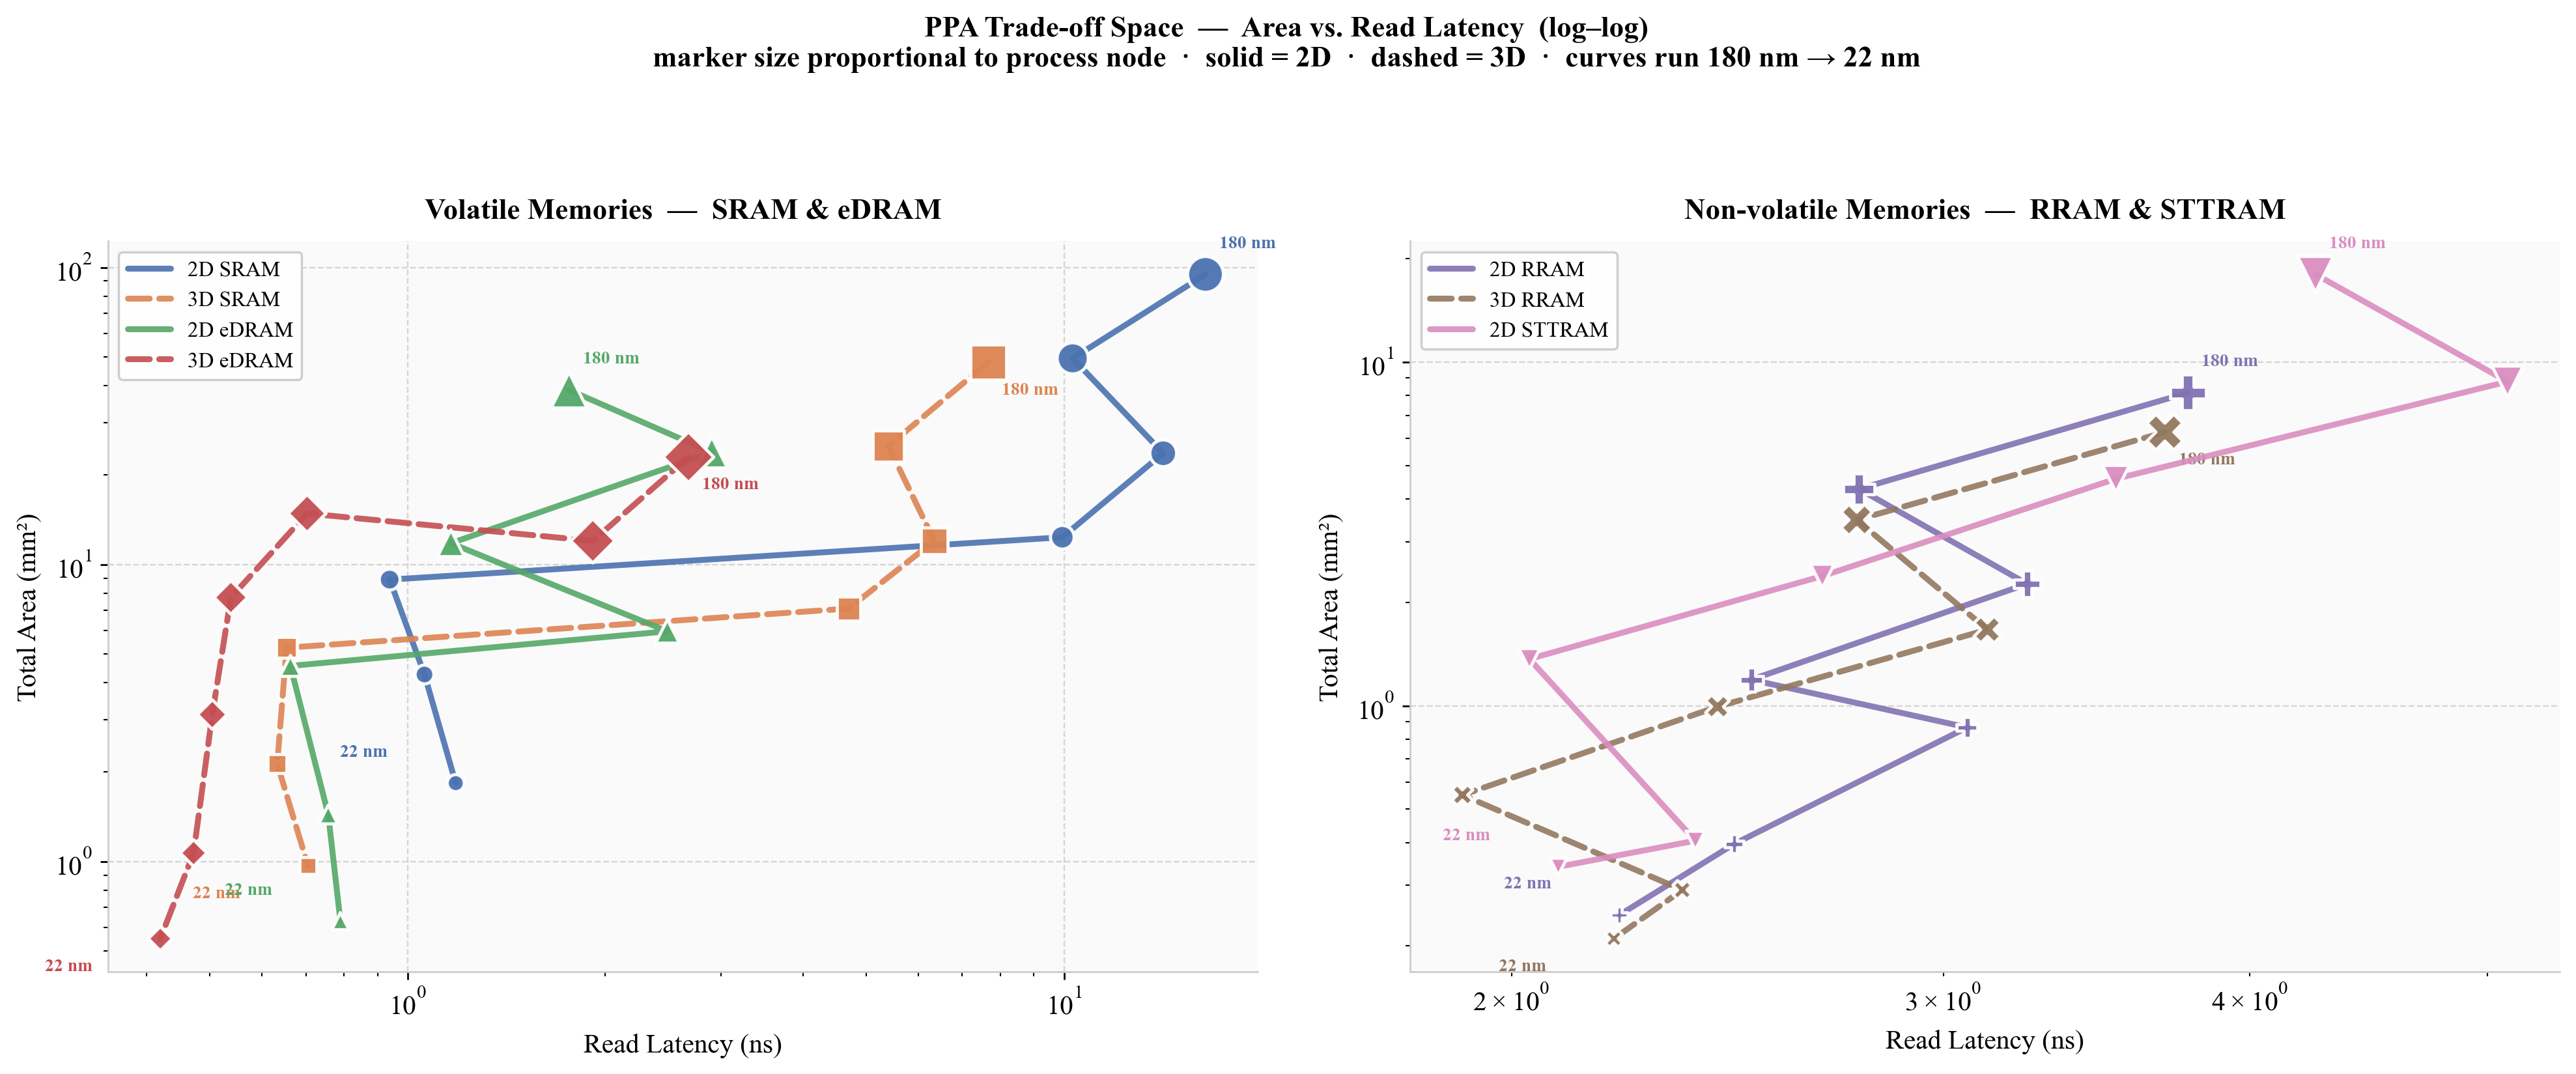
\includegraphics[width=0.92\textwidth]{ppa_scatter.png}
    \caption{PPA tradeoff space: area versus read latency for volatile and non-volatile memories.}
    \label{fig:ppa_scatter}
\end{figure*}

The volatile memory plot shows that 2D SRAM starts with large area and high latency at older nodes, but improves significantly as the node scales down. 3D SRAM reduces area and latency compared with 2D SRAM. 3D eDRAM occupies a favorable region with low area and low read latency at advanced nodes.

The non-volatile memory plot shows that RRAM and STT-RAM provide good area density, but their latency trends are more model-dependent. This reinforces the need to evaluate non-volatile memories separately from SRAM and eDRAM rather than ranking all technologies using a single metric.

\subsection{Radar PPA Analysis}

Fig.~\ref{fig:radars} presents radar charts at 90 nm, 45 nm, and 22 nm. These charts summarize six PPA dimensions: area, read latency, write latency, read energy, write energy, and leakage power.

\begin{figure*}[t]
    \centering
    \begin{subfigure}[t]{0.32\textwidth}
        \centering
        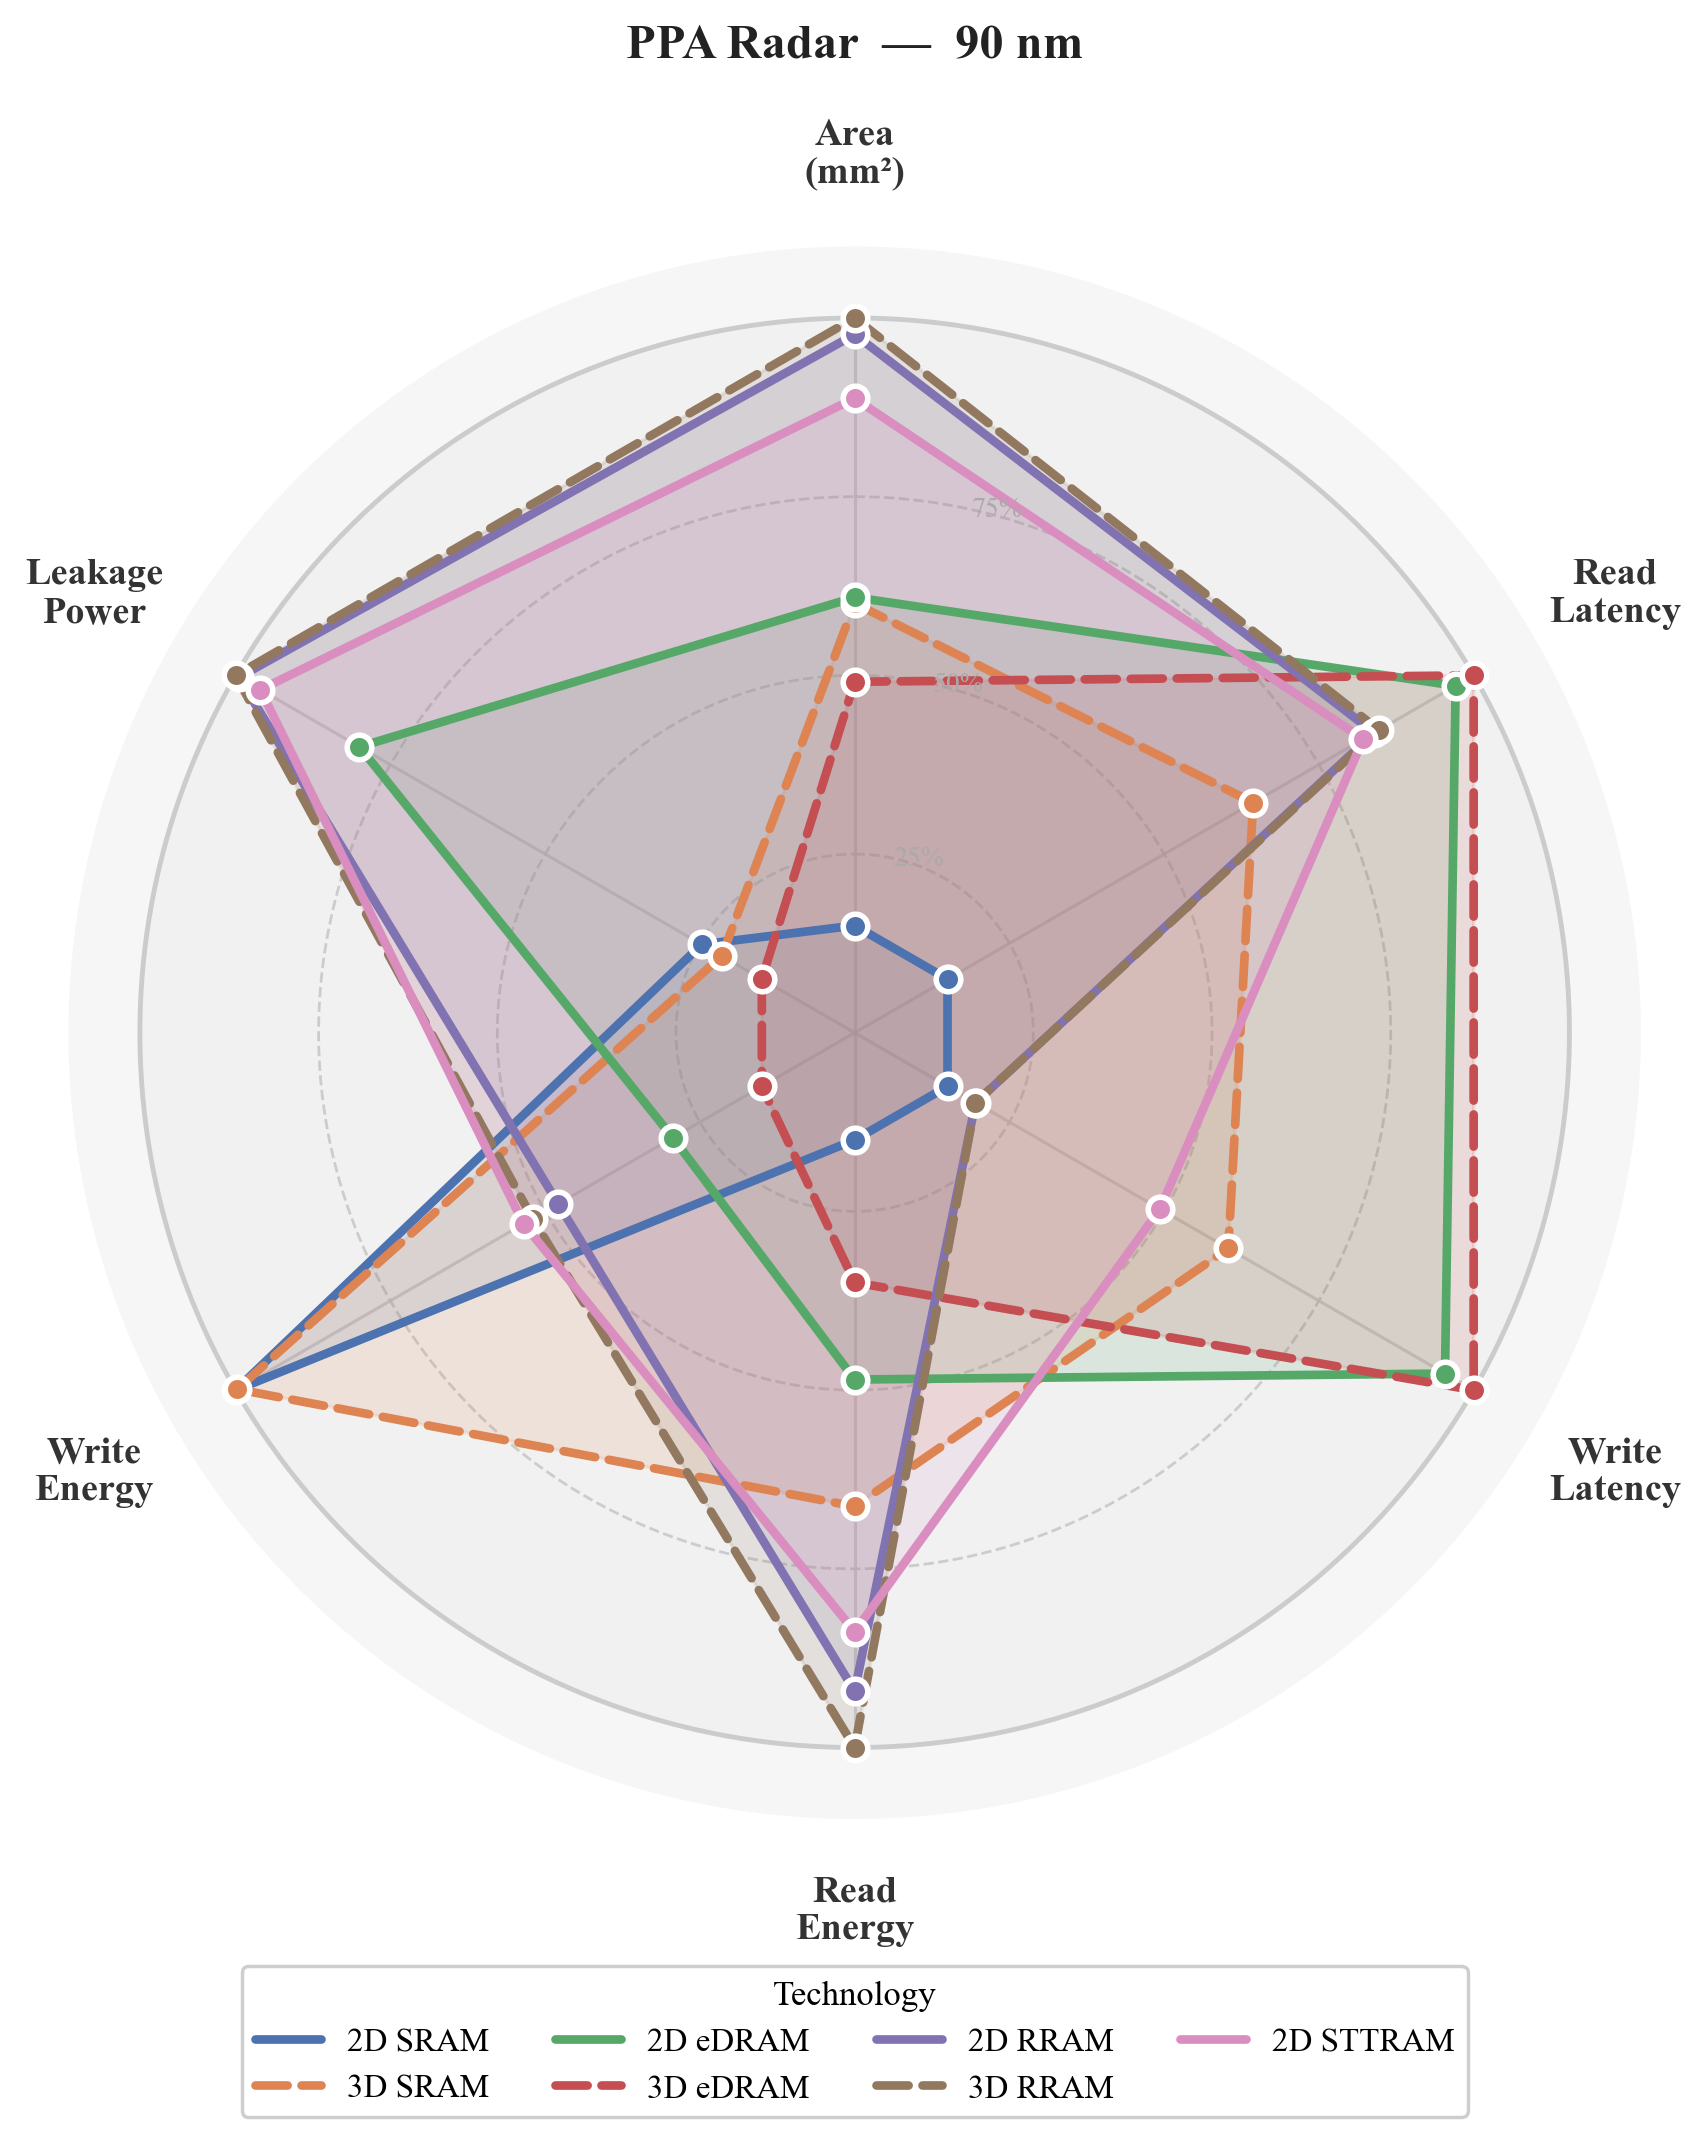
\includegraphics[width=\linewidth]{radar_90nm.png}
        \caption{90 nm}
    \end{subfigure}
    \begin{subfigure}[t]{0.32\textwidth}
        \centering
        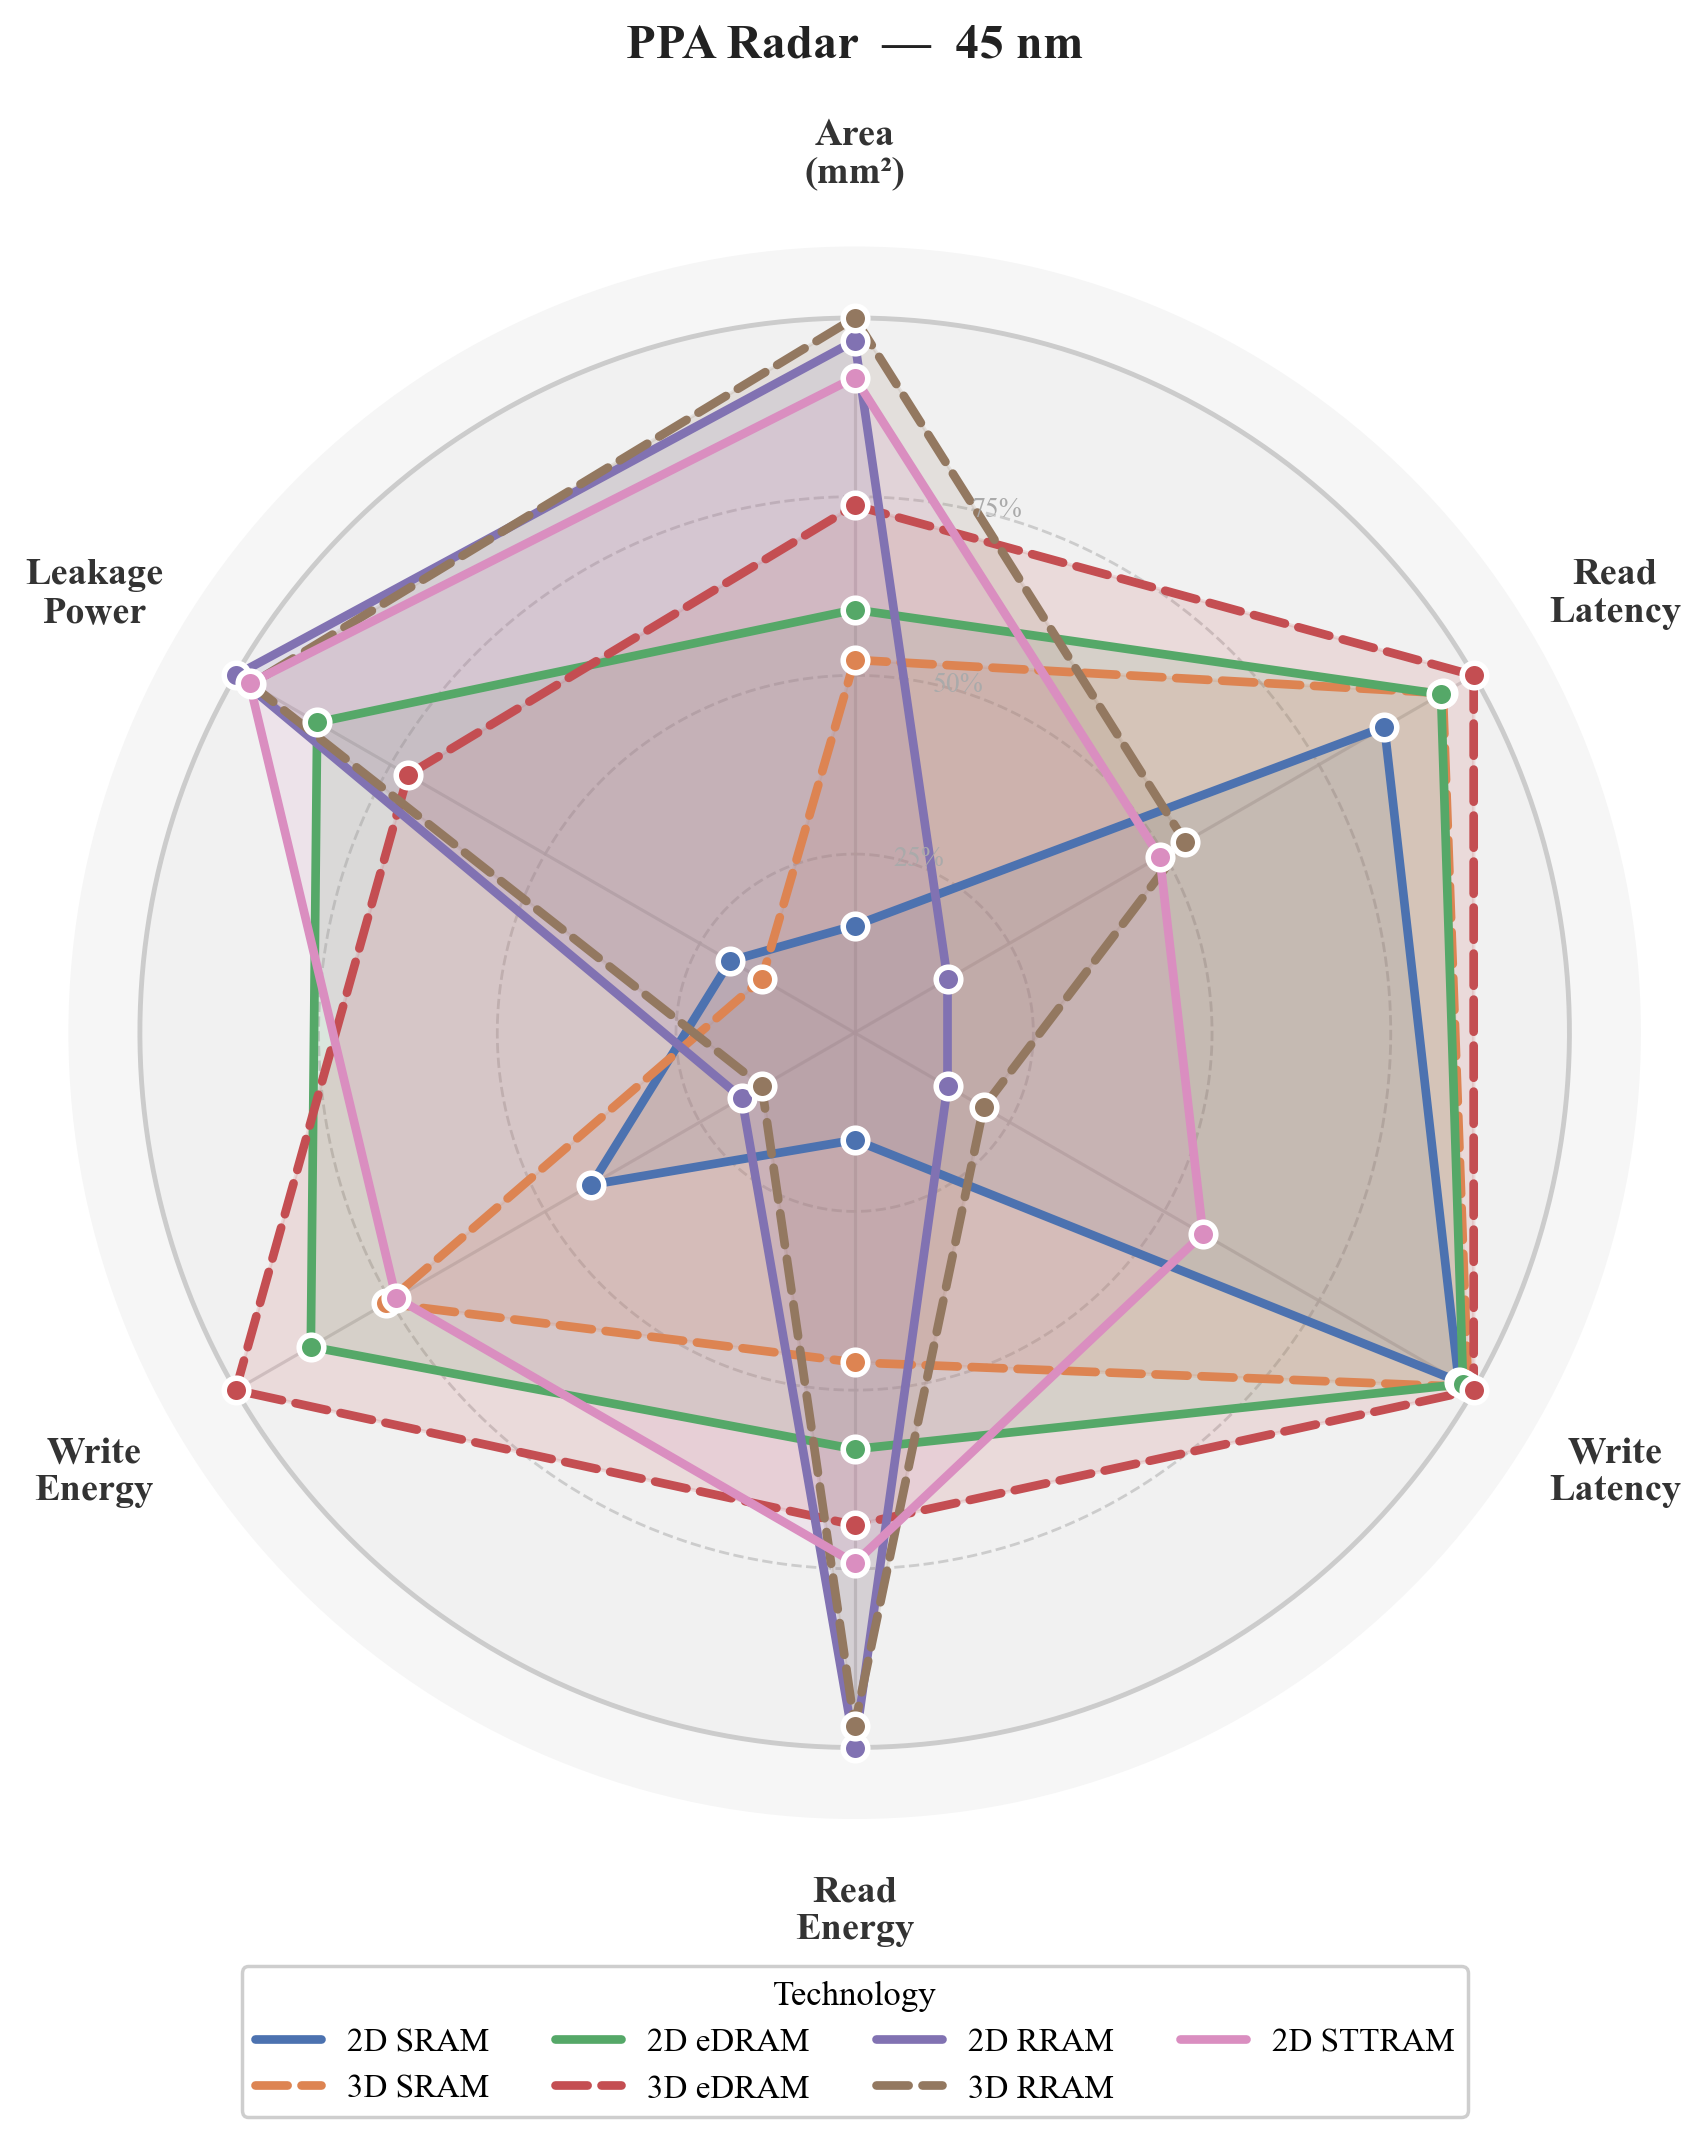
\includegraphics[width=\linewidth]{radar_45nm.png}
        \caption{45 nm}
    \end{subfigure}
    \begin{subfigure}[t]{0.32\textwidth}
        \centering
        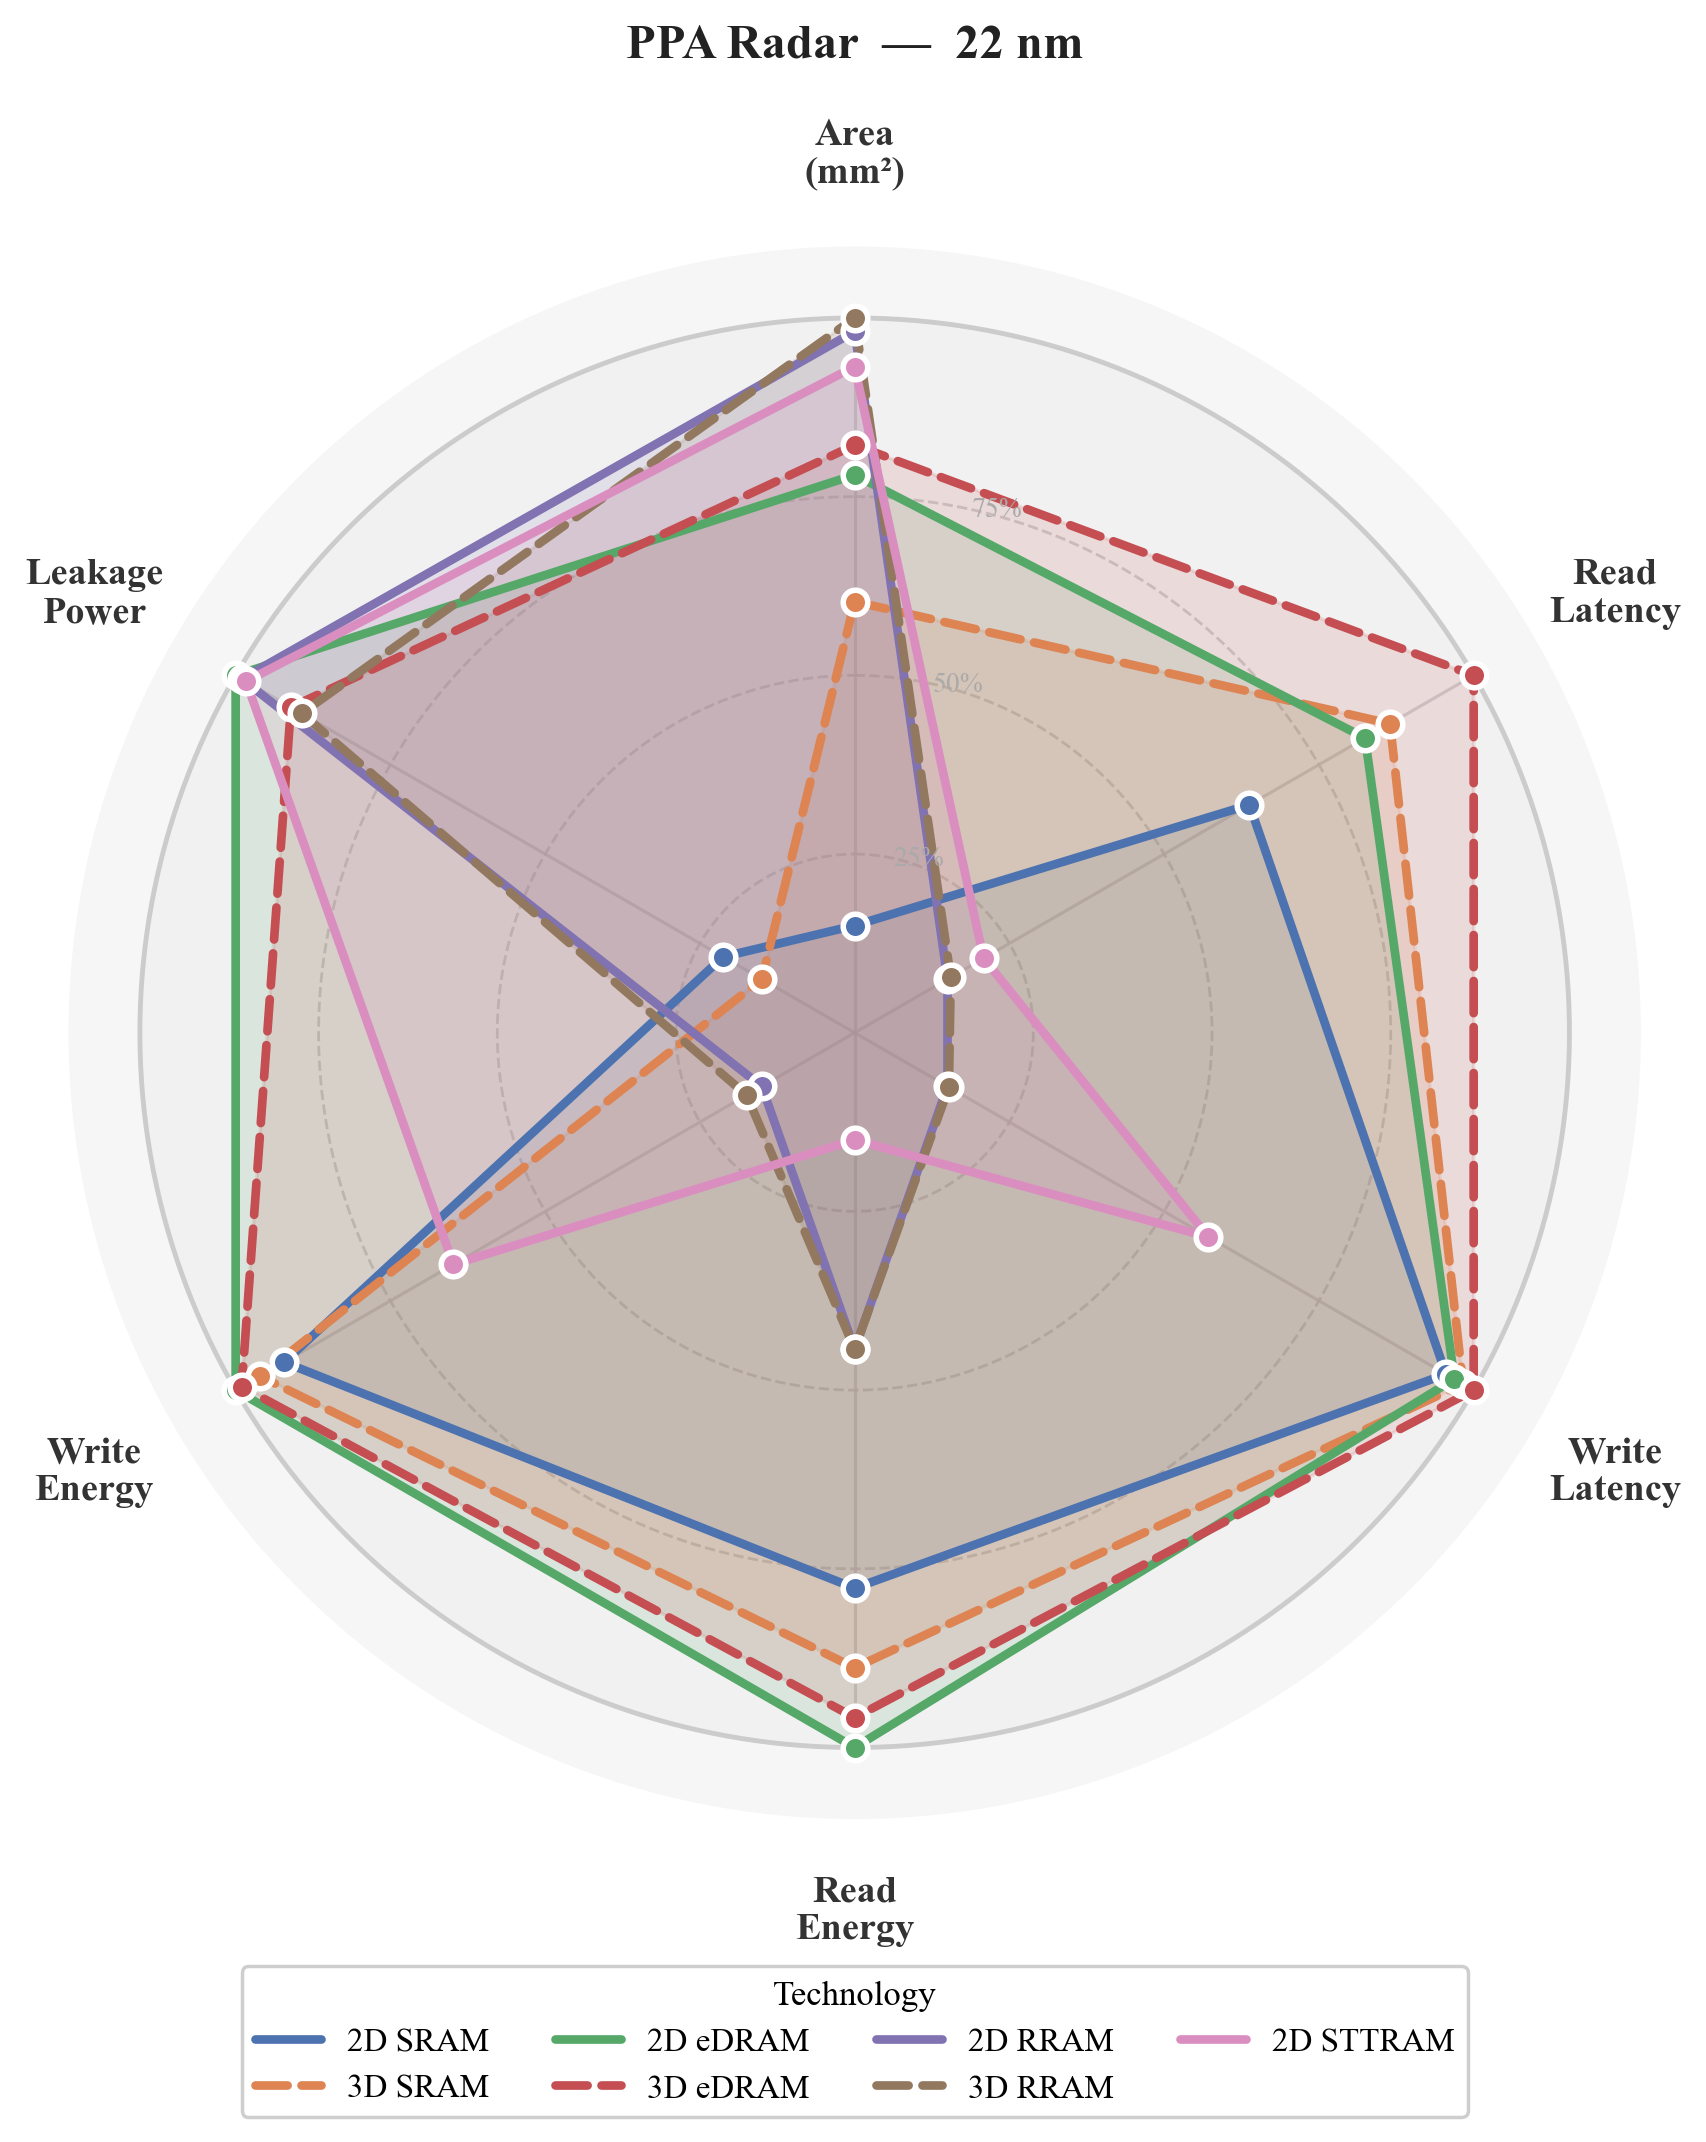
\includegraphics[width=\linewidth]{radar_22nm.png}
        \caption{22 nm}
    \end{subfigure}
    \caption{PPA radar comparison at representative process nodes.}
    \label{fig:radars}
\end{figure*}

The 90 nm radar plot shows clear separation between memory technologies. SRAM is weak in area and leakage, while eDRAM and 3D eDRAM show stronger latency and density characteristics. At 45 nm, the tradeoff becomes more balanced, and 3D eDRAM remains strong in read/write latency. At 22 nm, many technologies improve in area and energy, but leakage and write behavior still separate the technologies.

The radar plots make clear that no memory technology dominates all metrics. Instead, each technology has a different PPA profile. Therefore, the best choice depends on whether the application prioritizes density, latency, energy, leakage, or non-volatility.

\section{TSV Sensitivity Analysis}

\subsection{TSV Impact on Area}

Fig.~\ref{fig:tsv_area} shows the effect of TSV parameters on total area for 3D SRAM at 32 nm.

\begin{figure}[htbp]
    \centering
    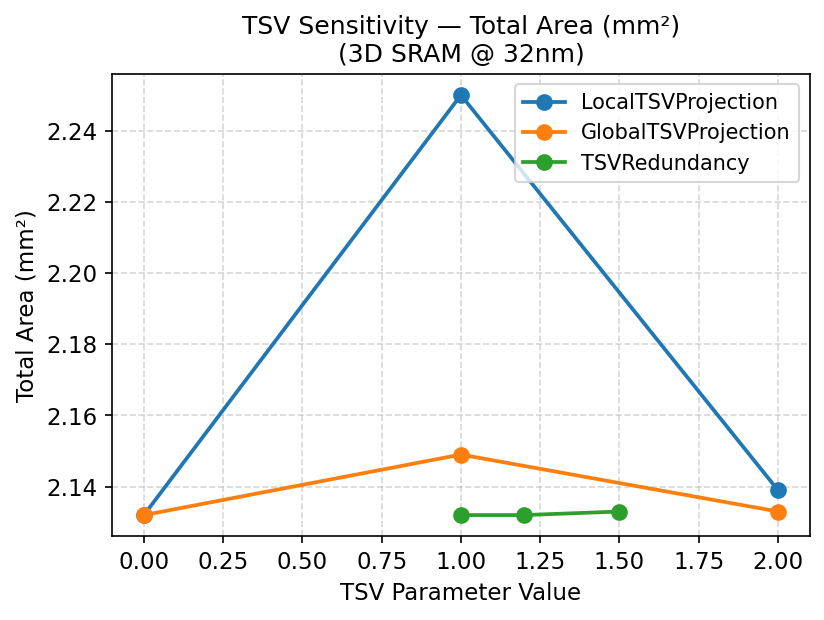
\includegraphics[width=0.48\textwidth]{fig07_tsv_sensitivity_area.png}
    \caption{TSV sensitivity analysis for total area of 3D SRAM at 32 nm.}
    \label{fig:tsv_area}
\end{figure}

Among the three TSV parameters, LocalTSVProjection has the strongest impact on area. When LocalTSVProjection increases from 0 to 1, the total area increases noticeably. This is because local TSVs are placed closer to the memory subarrays and directly affect local layout overhead. Their pitch and keep-out regions compete with bitcell and local interconnect area.

In comparison, GlobalTSVProjection causes only a small area change because global TSV overhead is distributed across a larger memory structure. TSVRedundancy has almost no visible area impact in this configuration. Overall, this result indicates that the local TSV assumption is the most important TSV-related factor for area estimation.

\subsection{TSV Impact on Read Latency}

Fig.~\ref{fig:tsv_latency} shows the read latency sensitivity of 3D SRAM at 32 nm under different TSV parameter values.

\begin{figure}[htbp]
    \centering
    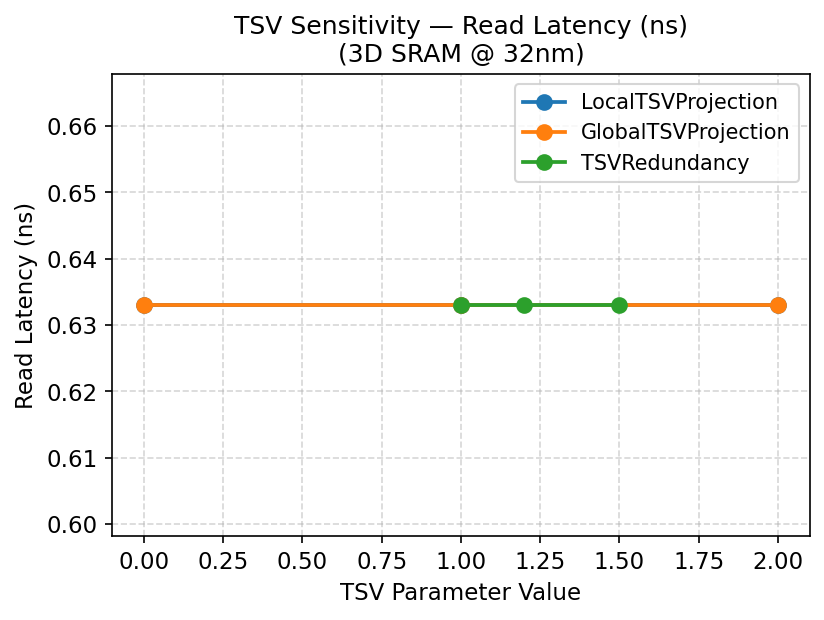
\includegraphics[width=0.48\textwidth]{fig08_tsv_sensitivity_read_latency.png}
    \caption{TSV sensitivity analysis for read latency of 3D SRAM at 32 nm.}
    \label{fig:tsv_latency}
\end{figure}

The read latency remains almost constant for all TSV settings. This means TSV delay is not the dominant critical path in this configuration. Instead, the main timing contribution is more likely from within-die routing, H-tree interconnect, and subarray access.

This result suggests that TSV assumptions have limited impact on system-level read latency for this 3D SRAM configuration. However, TSV assumptions still matter for area, especially through local TSV design.

\section{Cross-Technology Tradeoff Analysis}

The results show that no single memory technology is best for all metrics. Each technology has different advantages and limitations.

% \begin{table}[htbp]
% \caption{Summary of Memory Technology Tradeoffs}
% \begin{center}
% \begin{tabular}{p{0.18\linewidth} p{0.25\linewidth} p{0.27\linewidth} p{0.20\linewidth}}
% \toprule
% \textbf{Memory} & \textbf{Strength} & \textbf{Weakness} & \textbf{Best Use Case} \\
% \midrule
% SRAM & low intrinsic latency & large area and high leakage & refresh-free cache \\
% eDRAM & high density and low leakage & refresh required & area/power-sensitive memory \\
% 3D SRAM & reduced footprint vs. 2D SRAM & TSV and leakage overhead & density-improved SRAM \\
% 3D eDRAM & strong area and read latency & refresh and TSV overhead & high-density, fast memory \\
% STT-RAM & non-volatility and low standby power & higher write cost & non-volatile cache \\
% RRAM & density potential & model and parameter uncertainty & emerging NVM exploration \\
% \bottomrule
% \end{tabular}
% \label{tab:tradeoff}
% \end{center}
% \end{table}
\begin{table*}[t]
\caption{Summary of Memory Technology Tradeoffs}
\label{tab:tradeoff}
\centering
\renewcommand{\arraystretch}{1.15}
\setlength{\tabcolsep}{5pt}
\begin{tabularx}{\textwidth}{@{}
>{\RaggedRight\arraybackslash}p{0.13\textwidth}
>{\RaggedRight\arraybackslash}X
>{\RaggedRight\arraybackslash}X
>{\RaggedRight\arraybackslash}X
@{}}
\toprule
\textbf{Memory} & \textbf{Strength} & \textbf{Weakness} & \textbf{Best Use Case} \\
\midrule
SRAM & Low intrinsic latency and mature CMOS compatibility & Large area and high leakage & Refresh-free cache designs \\
eDRAM & High density and low leakage & Refresh and retention overhead & Area- and power-sensitive memory \\
3D SRAM & Smaller footprint than 2D SRAM & TSV and additional peripheral overhead & Density-improved SRAM cache \\
3D eDRAM & Strong area and read-latency performance under the fixed DESTINY setup & Refresh, TSV, and stacking overhead & High-density, latency-sensitive memory \\
STT-RAM & Non-volatility and low standby power & Higher write latency and write energy & Non-volatile cache exploration \\
RRAM & High density potential & Device-parameter and model uncertainty & Emerging NVM design-space exploration \\
\bottomrule
\end{tabularx}
\end{table*}


For latency-critical and area-critical systems, 3D eDRAM is one of the most promising options because it combines compact cell structure with stacking benefits. For leakage-sensitive applications, 2D eDRAM and RRAM-based options are attractive. SRAM remains useful when refresh overhead is not acceptable, but its leakage and area overhead are significant.

\section{Model Limitation and Interpretation Boundary}

Although DESTINY is useful for early-stage design-space exploration, its results should not be interpreted as exact silicon measurements. Several limitations should be considered.

First, the simulator relies on memory-cell parameter files and technology models. Emerging memory results such as STT-RAM and RRAM can be sensitive to assumed device parameters. Second, eDRAM refresh energy is not fully represented in the basic leakage comparison, so the power advantage of eDRAM may be partially reduced in real systems. Third, 3D integration is modeled at the architectural level, while real 3D IC implementation may involve additional thermal, mechanical, yield, and manufacturing constraints. Finally, the optimization target can strongly affect the selected memory organization, causing non-monotonic results.

Therefore, the strongest use of DESTINY is controlled relative comparison rather than absolute physical prediction.

\section{Conclusion}

This project uses DESTINY to compare 2D and 3D memory technologies across multiple process nodes. The results show that memory scaling is affected not only by process-node reduction, but also by memory cell structure, interconnect hierarchy, 3D stacking, TSV overhead, and optimizer-selected memory organization.

The process-node results show that area and read energy generally improve as technology scales. However, latency, write energy, and leakage can show non-monotonic trends due to internal organization changes selected by DESTINY. The heatmaps and radar plots further show that no memory technology dominates all PPA metrics.

Overall, 3D eDRAM provides strong area and read-latency advantages at advanced nodes, making it suitable for high-density and high-speed memory designs. 2D eDRAM and RRAM-based options are attractive for leakage- or density-sensitive applications. SRAM remains useful when refresh overhead is not acceptable, but it has higher area and leakage cost.

The layer-scaling analysis shows that stacking can improve area and EDP, especially for SRAM and eDRAM, but the improvement is not always monotonic. TSV sensitivity analysis further shows that LocalTSVProjection has the largest impact on 3D SRAM area, while read latency remains almost unchanged under different TSV assumptions.

In summary, DESTINY is most useful for controlled relative comparison and early-stage memory design exploration. The best memory technology depends on the target design priority: density, latency, energy, leakage, or non-volatility.

\appendices

\section{Contribution Table for Team Members}

\begin{table}[htbp]
\caption{Summary of Individual Contributions}
\begin{center}
\renewcommand{\arraystretch}{1.25}
\begin{tabular}{p{0.22\linewidth} p{0.68\linewidth}}
\toprule
\textbf{Member} & \textbf{Contribution} \\
\midrule
Zhengyu Liu & 
Worked on DESTINY simulation setup, configuration adjustment, process-node sweep, and extraction of area, latency, energy, and leakage data. Contributed to organizing raw simulation results and validating the consistency of output trends. \\
\midrule
Tiebing Tang & 
Worked on TSV sensitivity analysis and stacked-die improvement analysis, including layer count comparisons and EDP improvement interpretation. Contributed to generating TSV, layer-scaling, and heatmap figures. \\
\midrule
Yishu Wang & 
Worked on report writing, poster preparation, figure interpretation, conclusion development, and presentation organization. Contributed to methodology explanation, results discussion, PPA analysis, and final report formatting in IEEE style. \\
\bottomrule
\end{tabular}
\label{tab:contribution}
\end{center}
\end{table}

\section*{Acknowledgment}

The authors would like to express their sincere gratitude to Prof. Robert M. Radway for his instruction and guidance throughout ESE5760 Semiconductor Memory Devices and Circuit Design. His lectures and feedback helped us better understand memory device modeling, process-node scaling, and the design tradeoffs of 2D and 3D memory systems.

\begin{thebibliography}{00}

\bibitem{destiny}
M. Poremba, S. Mittal, D. Li, J. S. Vetter, and Y. Xie, ``DESTINY: A tool for modeling emerging 3D NVM and eDRAM caches,'' in \textit{Proc. Design, Automation \& Test in Europe Conference \& Exhibition (DATE)}, 2015, pp. 1543--1546.

% \bibitem{cacti3dd}
% K. Chen, S. Li, J. H. Ahn, J. B. Brockman, and N. P. Jouppi, ``CACTI-3DD: Architecture-level modeling for 3D die-stacked DRAM main memory,'' in \textit{Proc. Design, Automation \& Test in Europe Conference \& Exhibition (DATE)}, 2012.

% \bibitem{nvsim}
% X. Dong, C. Xu, Y. Xie, and N. P. Jouppi, ``NVSim: A circuit-level performance, energy, and area model for emerging nonvolatile memory,'' \textit{IEEE Transactions on Computer-Aided Design of Integrated Circuits and Systems}, vol. 31, no. 7, pp. 994--1007, 2012.

% \bibitem{cacti}
% N. Muralimanohar, R. Balasubramonian, and N. P. Jouppi, ``CACTI 6.0: A tool to model large caches,'' HP Laboratories, Tech. Rep. HPL-2009-85, 2009.

\end{thebibliography}

\end{document}